%%
%% Template of the department Very Large Business Applications,
%%    CvO University Oldenburg for scientific papers
%%
%% Created by Dipl.-Inform. Daniel Süpke
%%    For questions, comments, suggestions etc. send an email to:
%%    suepke@wi-ol.de or suepke@gmx.de
%%
%% Version: April 16, 2010
%%
%% Note: Has only been tested with pdflatex, not latex (dvi). Still, there is
%% theoretical support also for latex.
%%


\documentclass[11pt]{scrartcl}

%% packages
\usepackage[utf8]{inputenc}       % Standard for Linux
%\usepackage[latin1]{inputenc}    % Standard for Windows
\usepackage{ngerman}              % For German language
\usepackage{fancyhdr}
\usepackage{geometry}
\usepackage{ifpdf}
\usepackage{setspace}             % For line spread
\usepackage{enumitem}
\usepackage{caption}


%\usepackage{url}
%\usepackage[sorting=none]{biblatex}


% For pdflatex
\ifpdf
  % One of these two:
  \usepackage[pdftex]{graphicx}
  %\usepackage[pdftex]{epsfig}

  \usepackage[pdftex]{hyperref}
% For latex (dvi)
\else
  % One of these two:
  \usepackage[dvips]{graphicx}
  %\usepackage[dvips]{epsfig}

  % make the command \href from hyperref available as a 'print only'
  \newcommand{\href}[2]{#2}
\fi

%% Picture options
\graphicspath{{pictures/}}         % Default path to pictures used
\DeclareGraphicsExtensions{.png}   % More extensions can be added


%% Pagestyle options
\pagestyle{fancy}
%\lhead{}
%\chead{}
%\rhead{}
%\lfoot{Daniel Süpke}
%\cfoot{}
%\rfoot{}
\renewcommand{\headrulewidth}{0.4pt}

\bibliographystyle{base/plaindin} 

\geometry{a4paper,left=3cm,right=3cm}
%\geometry{a4paper,left=3cm,right=2.5cm}   % Please use these settings for a PhD-thesis




%% Document start
\begin{document}

%% Title page
\begin{titlepage}
 	\begin{centering}
	\begin{figure}[h!]
    \centering
    
\includegraphics[width=310pt]{pics/uol}    % Ggf. Copyright beachten - ansonsten nur für Gebrauch an der CvO
	\end{figure}
	\large DEPARTMENT FÜR INFORMATIK\\

  	\vspace*{2cm}
  
	\LARGE \textbf{Exposé\\}
	\vspace*{0.2cm}
  	\Large zur Bachelorarbeit\\
  	\vspace*{1cm}  
  

  %\emph{Bei Referaten noch mit Zusatz:} im Rahmen des..     % Insert correct type

  \end{centering}
  
  \vspace*{3cm}
  \begin{tabbing}
  xxxxxxxxxxxxxxxx\= \kill
  
  % Change me
  %\small Themensteller:\> Prof. Dr.-Ing. Jorge Marx Gómez\\
  \small \textbf{Betreuer: }\> Dr. Ute Vogel-Sonnenschein\\\\

  \small \textbf{Autor: }\>Cinddy Vannessa Canon Pasquel\\
  %\small \>Semesteranschrift\\
  %\small \>PLZ Wohnort:\\
  %\small \>Telefonnummer:\\
  \small \>cinddy.vannessa.canon.pasquel@uni-oldenburg.de\\\\
  \end{tabbing}
  \vspace*{1cm}
  \normalsize \centering Juni 2020
\end{titlepage}



%\thispagestyle{empty}
\newpage

\tableofcontents
\newpage


%\section*{Glossar}             % Alternatively a glossary package can be used
%\addcontentsline{toc}{section}{Glossar}
%\section*{Symbolverzeichnis}   % If needed
%\addcontentsline{toc}{section}{Symbolverzeichnis}
%\newpage

\listoffigures
\addcontentsline{toc}{section}{Abbildungsverzeichnis}
%\listoftables
%\addcontentsline{toc}{section}{Tabellenverzeichnis}
\newpage

%% Line spread
\onehalfspacing


% For large documents, instead of typing all the text inside here, it may be better
% splitting the content in multiple files and using \include or \includeonly

% Start of content
\section{Einleitung}
Die Erstellung dieser Bachelorarbeit findet innerhalb des Studiengangs Informatik der Fakult\"at II - Informatik, Wirtschafts- und Rechtswissenschaften an der Carl von Ossietzky Universit\"at Oldenburg statt.
Dieses Expos\'{e} soll eine kurze Einleitung in die durchzuf\"uhrende Bachelorarbeit darstellen.\\

Im Folgenden m\"ochte ich eine grobe Einf\"uhrung in die Thematik geben, die Zielsetzung, die Motivation und die Problemstellung meiner Bachelorarbeit beschreiben, eine aktuelle \"Ubersicht vorhandener Studien darlegen und abschlie{\ss}end meine vorl\"aufige Gliederung und Zeitplanung vorstellen.
\subsection{Einführung}
Die Struktur des Studienplans eines akademischen Bachelorprogramms an der Carl von Ossietzky Universität Oldenburg besteht aus vier verschiedenen Modulkategorien. Zum einen aus Basis- und Aufbaumodulen, die zu dem Pflichtbereich gehören und die wichtige Grundlage des Studiums vermitteln; zum zweiten aus Akzentssetzungsmodule, die Studierenden eine individuelle Ausrichtung geben können. Zusätzlich gibt es Professionalisierungs- und Praxismodule, die den Erwerb berufsbezogener und praktischer Kenntnisse stellen. Zulässt muss ein Abschlussmodul abgeschlossen werden. Master of Education und Master sind anderes aufgebaut aber auch für sie gibt es Abschlussarbeit.\\
Das Abschlussmodul ist eine vertiefende Prüfungsleitung, die von den Studenten als Voraussetzung für die Qualifikation des Abschlusses entwickelt wurde\cite{BScInf:2020}.\\

Bei der Anfertigung der Abschlussarbeit muss die\textbackslash der Studierende zunächst ein Thema für ihre\textbackslash seine Forschungsarbeit finden, welches für sein Studienprogramm relevant sein muss. Es ist möglich, dass Studierende in Absprache mit einer Gutachterin bzw. einem Gutachter selbst ein Thema für eine Abschlussarbeit wählen können, oder dass, es durch eine Einrichtung au{\ss}erhalb der Universität ausgeführt werden kann\cite{Boles:2015}.\\

Das Department für Informatik ist in vier Fachrichtungen aufgegliedert: Theoretische Informatik, Praktische Informatik, Angewandte Informatik und Technische Informatik, und jede davon ist nochmal in verschiedene Vertiefungsrichtungen unterteil. Insgesamt gibt es zur Zeit siebzehn Abteilungen\cite{SpeInf:2020}. Jede Abteilung setz sich aus Professoren und wissenschaftliche Mitarbeiter zusammen, die eine Forschungsgruppe bilden und für die von ihr durchgeführten Projekte verantwortlich sind.\\
Für Abschlussprojekte, die an der Universität entwickelt wurden, sollte jede Abteilung des Departments für Informatik auf einer Abteilungs-eigenen Website, aktuelle Themen für Abschlussarbeiten veröffentlichen oder beschreiben, wie Studierende in der entsprechenden Abteilung ein Thema erhält\cite{Boles:2015}.\\

Der Zugang zu Informationen über die Abschlussthemen sollte von dem Department für Informatik gewährleistet werden, indem es eine standardisierte Form der Suche anbietet, welche den Universitätsmitarbeitern ermöglicht, die veröffentlichten Informationen effizient zu aktualisieren, und Studierende ermöglicht, ihre persönlichen Interessen zu berücksichtigen. Die aktuelle Lösung, alle Abschlussthemen auf einer zentralen Website zu verknüpfen, hat sich nicht bewährt und sollte durch diese Arbeit abgelöst werden.

\newpage
\subsubsection{Zielsetzung}
Abschlussarbeiten. In diesem Zusammenhang sollte klargestellt werden, welche Kriterien sind für die Suche nach einem Forschungsthema relevant und unter welchen Parametern kann der aktuelle Prozess der Veröffentlichung und Zuordnung von Abschlussarbeitsthemen optimiert werden. Diese Informationen werden für den Entwurf und Implementierung einer Softwareanwendung berücksichtigt, mit der Studierende nach Themen von Abschlussarbeiten suchen und Mitarbeiter des Fachbereichs Informatik diese zuweisen und verfolgen können.
\section{Motivation}
Die Suche nach Abschlussthemen durch Studierende ist nicht einfach.  Das umfangreiche Angebot an Spezialisierungen bzw. Abteilungen des Departments für Informatik ermöglicht es den Studenten, sich mit dem Bereich zu befassen, der sie am meisten anspricht. Es gibt jedoch zahlreiche Forschungsthemen, die sogar zu verschiedenen Studienbereichen gehören können, wie bei Projekten der Abteilung Didaktik der Informatik - Fachgebiet Angewandte Informatik, wo Kenntnisse der Mikrorobotik / Regelungstechnik und Softwaretechnik, die Teil der Fachrichtungen Technische Informatik bzw. Praktische Informatik sind, erforderlich sein können.\\

Auf Grundlage der obigen Ausführungen werden die folgenden Fragestellungen aufgegriffen:

\begin{itemize}
	\item Welche Suchkriterien verwenden Studierende bei der Suche nach Abschlussarbeitsthemen in Begleitung mit wissenschaftlicher Mitarbeitern des Departments für Informatik?
	
	\item Welche Elemente sind für die Mitarbeitern des Departements für Informatik relevant, um die Verwaltung der zugewiesenen Projekte zu gewährleisten?
\end{itemize}

Diese Arbeit muss eine Lösung für die Probleme des Departments für Informatik bei der Suche, Zuordnung und Verwaltung von Abschlussarbeiten bieten. Basierend auf den Bedürfnissen von Studenten und akademischen Mitarbeitern und unter Verwendung der technologischen Werkzeuge, die die Universität anbietet.
\subsection{Problembeschreibung}
Derzeit posten die Abteilungen die verfügbaren Forschungsthemen, die als Abschlussarbeiten gelten können, in den Pinnwänden der Fakultätsbüros, sodass interessierte Studierende an der Universität sein müssen, um über diese Themen informiert zu werden.
Einige Abteilungen veröffentlichen die Themen zusätzlich auf der Website der Universität, es gibt eine zentrale Seite und da drunter Seiten für Abteilungen. Die Mitglieder der Abteilung müssen dann ständig auf die Aktualisierung der Projekte auf der Website achten aber nicht jeder Mitarbeiter hat Zugangsrechte auf die Aktualisierung des Inhalts der Website. Es ist nicht immer klar, welche Projekte bereits in Bearbeitung sind und welche noch verfügbar sind.\\

Andere Abteilungen wie Eingebettete Hardware- / Software-Systeme bitten an Studierende, die an Abschlussarbeitsthemen interessiert sind, eine formlose Bewerbung mit   den bisher belegten Modulen, persönlichen Kenntnissen und Interessen, an einen wissenschaftlichen Mitarbeiter der Abteilung zu senden. Dieser wird Ihnen dann mögliche Themen zukommen lassen und bei Bedarf einen Termin organisieren\cite{EHS:2020}.
Obwohl die Studierenden auf diese Weise eine persönliche Beratung erhalten, hängen die Antwortzeiten von der Verfügbarkeit der Mitarbeiter der Abteilung ab, und es kann sein, dass die angebotenen Projekte für den Studenten nicht von Interesse sind, was die Suche nach einem Forschungsthema weiterhin verzögern würde. Die Kommunikation erfolgt über Emails, die übersehen werden können und die nicht direkt zu einem Projekt verknüpft werden können, um die effektive Verwaltung der Abschlussarbeit zu gewährleisten.\\

Die aktuelle Art und Weise, in der die als Abschlussarbeit verfügbaren Forschungsthemen veröffentlicht werden, ermöglicht es den Studierenden nicht, eine schnelle, effiziente und personalisierte Suche entsprechend den Bedürfnissen der einzelnen Studierenden durchzuführen. Für die Mitarbeiter der Abteilung ist es derzeit nicht effizient, die Veröffentlichung verfügbarer Themen aufrechtzuerhalten und Informationsanfragen von Studenten weiterzuverfolgen.\\
Darüber hinaus hat das Department keinen Überblick darüber, wie viele Abschlussarbeiten derzeit angeboten werden und wie viele gesucht werden, sodass das Risiko besteht, dass sich der Abschluss der Studierenden durch eine lange Suchzeit verzögert.
\subsection{Stand der Forschung}
Im Bereich der Durchführung eines Studienprojekts wurde 2009\cite{Watat:2019} ein Lösungsvorschlag für das Problem der Suche nach Forschungsprojekten am DfI vorgelegt. Dieser Vorschlag wurde als Webanwendung konzipiert, die der Website der Universität hinzugefügt wurde. Dort müssen die Mitarbeiter der Abteilung Informationen aus Forschungsprojekten eingeben, die sowohl von Universitätsmitarbeitern als auch von externen Benutzern konsultiert werden können.
Die Webanwendung wurde mit HTML, CSS und Java sowie mit der MySQL-Datenbank programmiert. Die Suche erfolgt anonym, es erfolgt keine Authentifizierung.\\

Einige der Themen für Forschungsprojekte, die als Abschlussprojekte abgeschlossen werden können, werden derzeit auf der Website der Universität veröffentlicht. Die Informationen können öffentlich eingesehen werden, und da keine Authentifizierung vorliegt, ist es nicht möglich zu wissen, wie viele Personen an den Themen interessiert sind, oder zusätzliche Ma{\ss}nahmen zur Konsultation durchzuführen.\\

Die Universität nutzt die Stud.IP-Arbeitsumgebung, um die interne Kommunikation zwischen Fakultät und Studierenden zu verwalten. Dafür arbeiten die für die Verwaltung der Plattform zuständigen Mitarbeiter ständig an Tools und Funktionen, die die Benutzerinteraktion verbessern.
Stud.IP ist eine kostenlose, Open Source Softwareplattform, deren Hauptprogrammiersprache PHP ist\cite{SIPPHP:2020}. Unter diesen Merkmalen ist es möglich, die Software- und Programm-Widgets-Anwendungen als Ergänzung zur Hauptplattform herunterzuladen.\\
Als Open-Source-Software ist Stud.IP lizenzkostenfrei\cite{SIPOS:2020}, d.h. jeder kann sich die Software herunterladen, installieren und unbegrenzt nutzen. Entwickelt wird die Software von der Stud.IP-CoreGroup, der aktiven Entwicklungsgemeinschaft, einer Gemeinschaft von Betreibereinrichtungen, der data-quest GmbH sowie dem Hochschulverein ELAN e.V.\\

In letzter Zeit wurden Funktionen für die Stud.IP-Umgebung der Universität aufgenommen, mit denen Fragebögen (VIPs) und Umfragen (Stoodle) offen oder anonym durchgeführt werden können und deren Informationen zur Erstellung von Statistiken verwendet werden können.
\subsection{Aufgabenstellung}
In Anbetracht der Vorteile von Stud.IP, wo bereits eine Struktur installiert ist, welche die Authentifizierung von Benutzern verwaltet und deren Kommunikation ermöglicht, wird die Softwareanwendung als Stud.IP-Plugin entwickelt, das der Plattform hinzugefügt wird und von Benutzern je nach Profil verwendet werden kann: Tutor oder Dozent.\\

Für Benutzer mit einem Tutor-Profil wird eine Übersicht erstellt, in der sie abhängig von den ausgewählten Auswahlkriterien nach Abschlussarbeiten suchen können.

Benutzer mit einem Dozent-Profil verfügen über eine Übersicht, in der sie Abschlussarbeitsthemen hinzufügen, ändern oder löschen können.

\subsubsection{Vorläufige Datenstruktur}
Eine Fakultät kann mehrere Departments haben, jedes Department kann aber nur zu einer Fakultät gehören und es kann verschiedene Fachrichtungen besitzen.
Jede Fachrichtung kann nur zu einem Department zugeordnet werden und kann in mehrere Abteilungen unterteilt werden, wobei eine Abteilung nur zu einer Fachrichtung gehören kann.
Mehrere Betreuer können einer Abteilung zugehörig sein aber ein Betreuer ist jeweils nur einer Abteilung zugeordnet.\\

Ein Thema besteht aus einem Identifikator, einem Namen, einer Beschreibung und ein Veröffentlichungsdatum. Es wird in einer Sprache geschrieben und wird einer Forschungsart zugeordnet: praktisch oder theoretisch. Ebenso besitzt das Thema einen Wert für den Status, wie zum Beispiel reserviert oder in Bearbeitung. Au{ss}erdem werden für das Thema verschiedenen Kompetenzen vorausgesetzt, welche wiederum Voraussetzungen mehrerer Themen sein können.\\
Sollte sich eine Studierende für ein Thema interessieren, kann sie es reservieren. Daraufhin kann ihr das Thema von einem Dozenten zugeordnet werden.\\

Die vorläufige Entitäten und ihren Beziehungen werden in folgender Abbildung vorgestellt:\\


\cleardoublepage
\begin{figure}[hp]%[H]
    \centering
    %\textbf{Your title}\par\medskip
    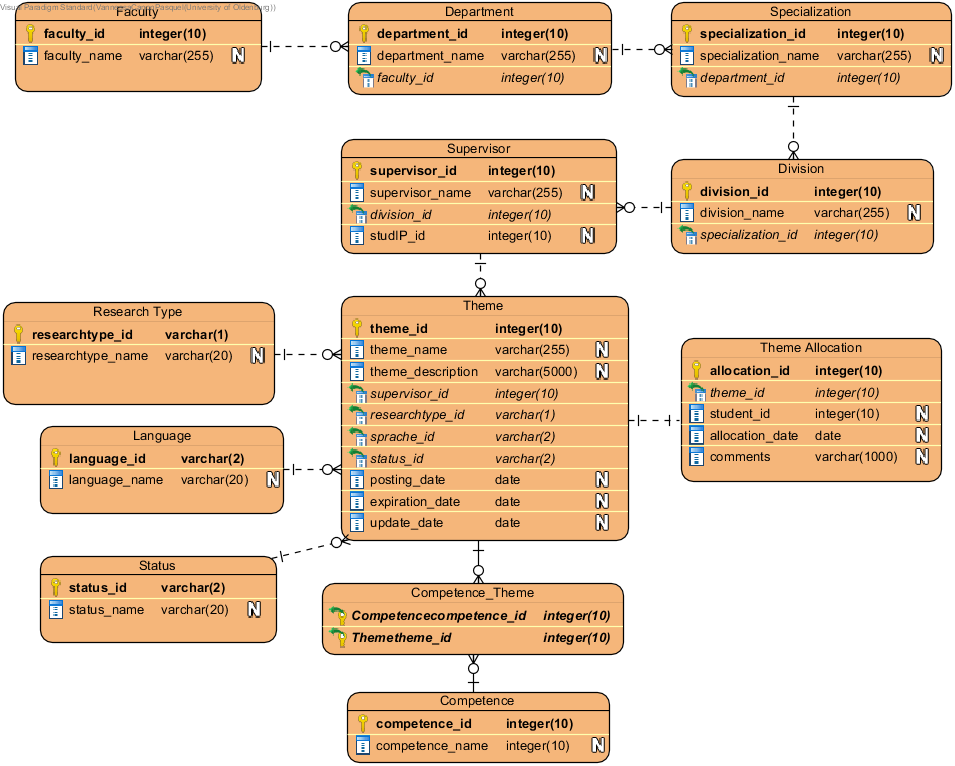
\includegraphics[height=12.5cm,keepaspectratio]{pics/ER_model}\\
    \caption{ER-Modell}
\end{figure}


\subsubsection{Definition von Suchkriterien}
Damit die Ergebnisse den Erwartungen der Studierenden so genau wie möglich entsprechen, wird eine Umfrage auf Basis der vorläufigen Datenstruktur durchgeführt.
In der Umfrage wird gefragt, welche Kriterien sind für die Studierenden relevant, wenn sie nach Themen für Abschlussarbeiten suchen und auch welche zusätzliche Funktionalitäten wären für die Softwareanwendung gewünscht.\\

\newpage
\textbf{Vorläufige Umfrage:}\\

Welche Kriterien sind für Sie relevant, bei der Suche nach Themen für Abschlussarbeiten:
	
	\begin{itemize}
	\item Studienabschluss
	\item Studiengang
	\item Fakultät
		\begin{itemize}[noitemsep]
			\item Department
			\item Fachrichtung
			\item Abteilung
			\item Betreuer
		\end{itemize}
	\item Forschungsart: Theoretisch, Praktisch
	\item Projekte ansehen
		\begin{itemize}[noitemsep]
			\item Verfügbare
			\item Reservierte
			\item Abgeschlossene
		\end{itemize}
	\item Angeforderte Kompetenzen: JAVA, SQL, Android, IoT, ERP{...}
	\item Sprache
	\item Veröffentlichungsdatum von - bis
	\item Ähnliche Projekte
	\item Andere:
	\end{itemize}
Gewünschte Funktionalitäten:
	
	\begin{itemize}
	\item Mehr Information über das Thema anfordern
	\item Projekt als Favorit merken
	\item Thema reservieren/befreien
	\begin{itemize}[noitemsep]
		\item Mehrere Projekte reservieren
		\item Projekte können von mehreren Studierenden reserviert werden
	\end{itemize}
	\item Andere:	
	\end{itemize}

\subsubsection{Entwurf der Softwareanwendung}
Benutzer können nach der Authentifizierung auf Stud.IP auf die Softwareanwendung-Plugin zugreifen.\\
Die Anwendung wird in PHP entwickelt, da dies die Hauptprogrammiersprache von Stud.IP ist.
Die Benutzeroberfläche enthält grafische Steuerelemente wie Button, Dropdown List, Text Box und Check Box, und es wird in ein Suchabschnitt im linken Bereich der Anwendung und ein Anzeigeabschnitt im rechten Bereich unterteilt, in dem die aus der Datenbank erhaltenen Ergebnisse gemä{\ss} den vom Benutzer ausgewählten Kriterien aufgelistet werden. Gruppen können zusammengeklappt und  aufgeklappt werden.\\

Wenn einen der Datensätze selektiert wird, werden zusätzliche Informationen zum ausgewählten Thema angezeigt, sodass der Benutzer das Abschlussarbeitsthema reservieren kann. Der Status des Themas wird in reserviert geändert, wodurch ein Datensatz in der Themenzuordnungstabelle generiert wird.\\
Die ausgewählten Filter, die Anzahl der abgerufenen Datensätze der Abfrage und eine Option zum Sortieren der Ergebnisse werden im Anwendungsheader angezeigt
Paginierung wird am Ende der Seite eingefügt, um eine gro{\ss}e Anzahl von Datensätzen zu unterstützen.\\

Die folgenden Bilder zeigen das vorläufige Design der Suche Übersicht. Anhang A enthält zusätzliche Bilder des Entwurfs nach dem Anwenden von Filtern.

\begin{figure}[hp]%[H]
    \centering
    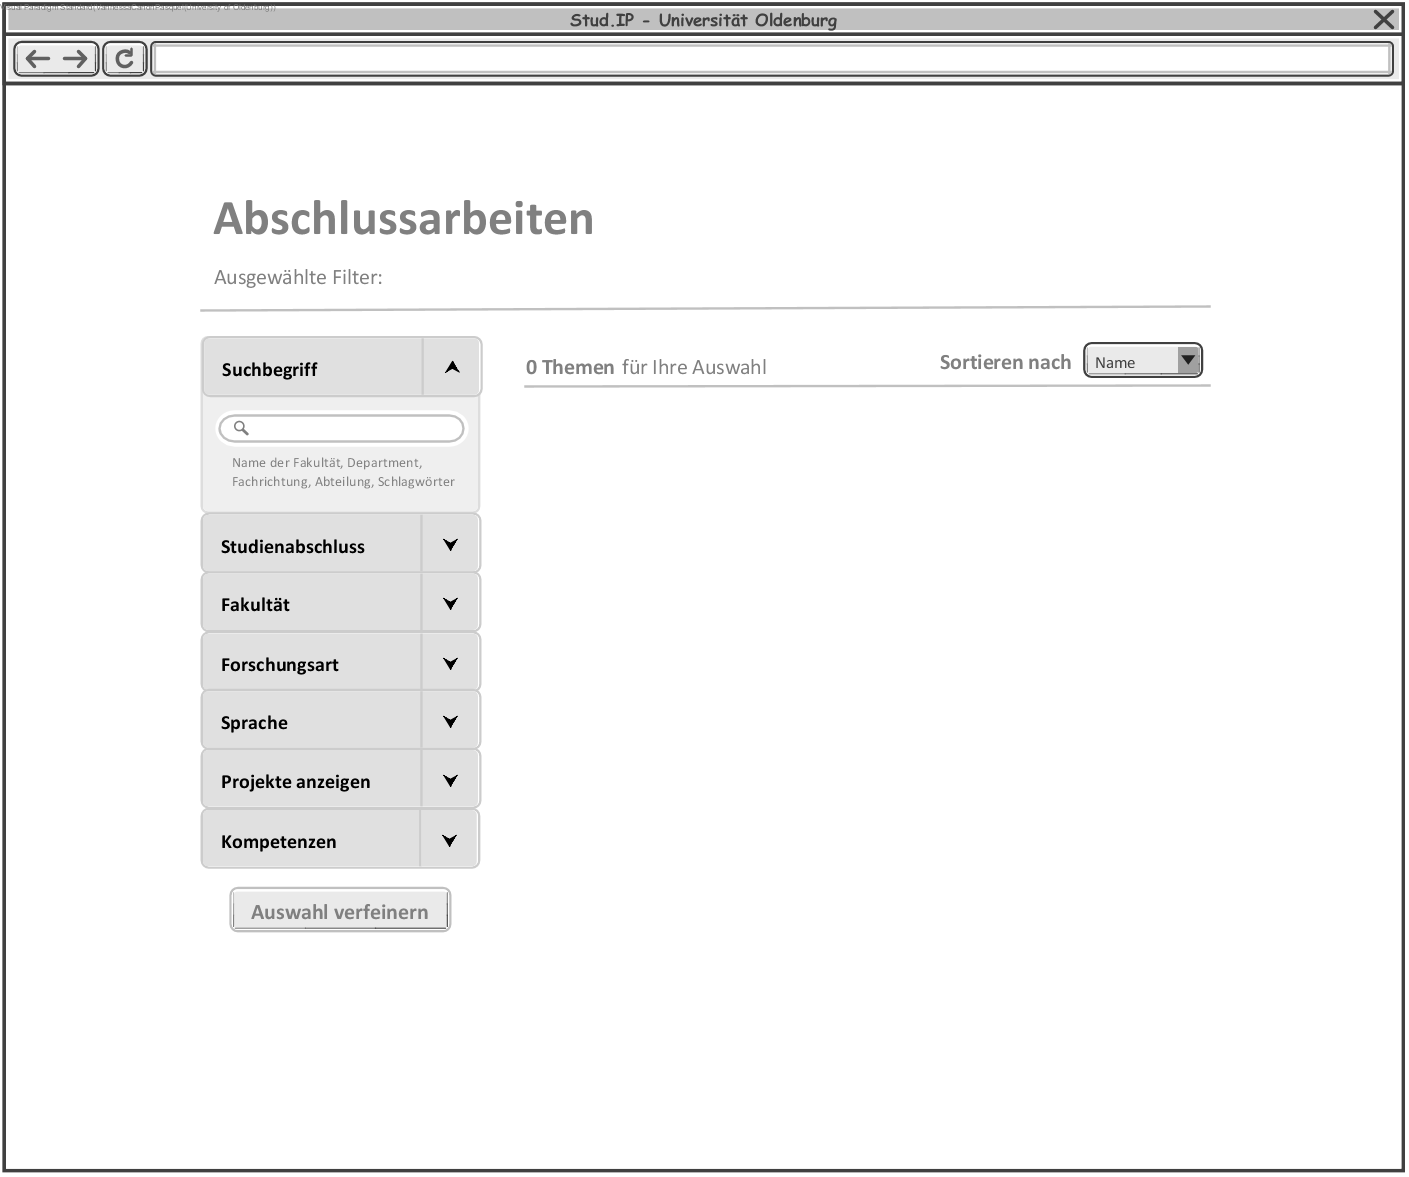
\includegraphics[height=7.5cm,keepaspectratio]{pics/app_collapsed}\\
    \caption{Suchkriterien zusammengeklappt}
\end{figure}

\cleardoublepage
\begin{figure}[hp]%[H]
    \centering
    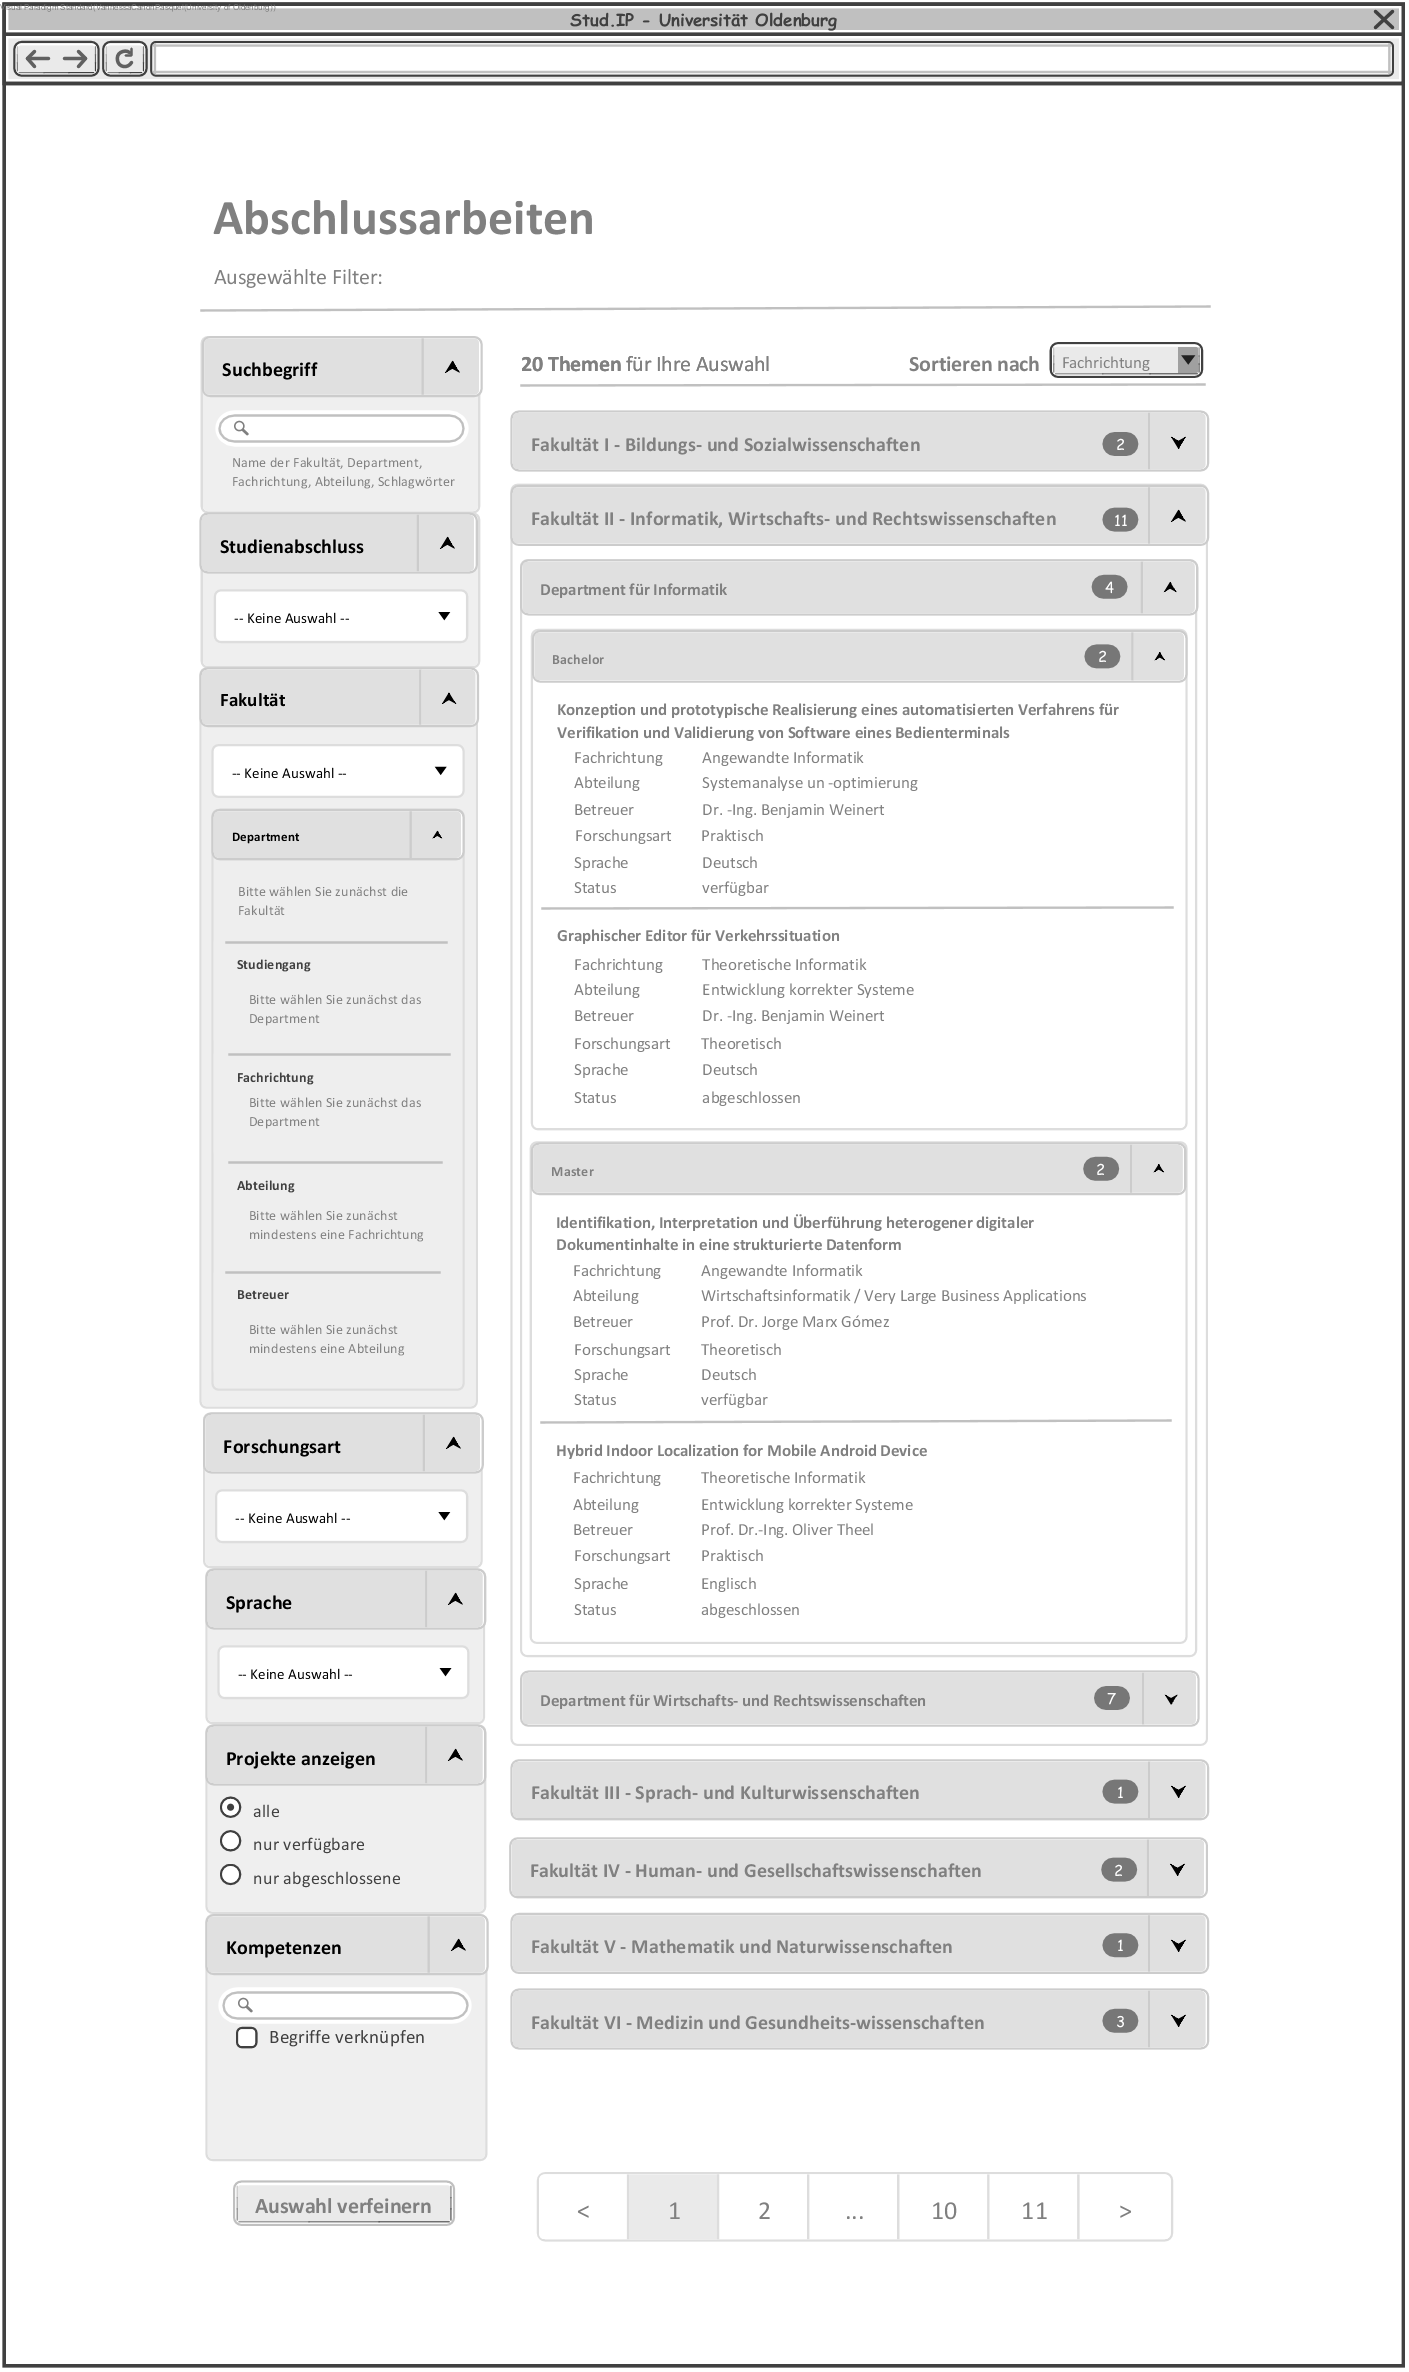
\includegraphics[height=20.5cm,keepaspectratio]{pics/app_expanded}\\
    \caption{Suchkriterien aufgeklappt - ohne Filter}
\end{figure}

\cleardoublepage
Zusätzlich wird eine Grundansicht für die Erstellung, Änderung und Beseitigung von Forschungsthemen durch Benutzer mit einem Dozent-Profil hinzugefügt. Dort werden Name, Beschreibung, Forschungsart, Sprache, Status und Ablaufdatum definiert. Nach der Erstellung wird das Veröffentlichungsdatum gespeichert.
Das Forschungsthema wird direkt der Abteilung des Benutzers zugewiesen, es kann jedoch definiert werden, wer der Betreuer ist.\\

Der Benutzer kann den Status des Themas ändern und festlegen, ob er akzeptiert, dass es von mehreren Benutzern reserviert werden kann, falls mehr als ein Benutzer an einem Thema interessiert ist, aber schließlich nur einer von ihnen es annehmen möchte. Ein Thema kann nur einem Benutzer zugewiesen werden.
Nachdem ein Thema geändert wurde, das Aktualisierungsdatum gespeichert.
  
\section{Rahmenbedingungen}

Ein Testsystem mit dem Stud-IP Projekt wird genutzt um das Projekt lokal zu entwickeln.
\section{Vorläufige Gliederung}

\begin{legal}[noitemsep]
\item Einleitung
	\begin{legal}
	\item Einführung und Zielsetzung
	\item Motivation
	\item Problembeschreibung
	\item Stand der Forschung
	\item Aufgabenstellung
	\end{legal}
\item Struktur des Departments für Informatik
	\begin{legal}
	\item Fachrichtungen
		\begin{legal}
		\item  Abteilungen
			\begin{legal}
			\item  Leitung
			\item  Betreuer
			\item  Veröffentlichung und Zuweisung von Abschlussarbeiten
			\end{legal}
		\end{legal}
	\end{legal}
\item Anforderungsanalyse
	\begin{legal}
	\item Ergebnisse der Umfrage und Datenanalyse
	\item User Stories
	\item Technische Anforderungen
	\item Definition der Suchkriterien und Suchalgorithmus
	\item Modellierung
		\begin{legal}
		\item  Entitäten und Beziehungen der Datenbank
		\item  Benutzeroberfläche
			\begin{legal}
			\item  Tutor
			\item  Dozent
			\end{legal}
		\end{legal}
	\end{legal}
\item Entwicklung und Implementierung
	\begin{legal}
	\item Herausforderungen
	\item Tests
	\item Ergebnisse
	\end{legal}
\item Fazit
\item Anhang
\item Literaturverzeichnis
Erklärung
\end{legal}
\chapter{Vorläufige Zeitplanung}
gemäß den Leitfaden zur Durchführung von Bachelor-Abschlussarbeiten\cite{Boles:2015}, die Dauer der Bachelorarbeit beträgt vier Monate.\\
Der erste Teil der Zeit wird genutzt um das Projekt vollständig zu strukturieren. In der Einarbeitungsphase, wird das notwendige fehlende Wissen erworben.\\
Die dritte Phase befasst sich mit der Entwicklung der Softwareanwendung sowohl auf Datenbank- als auch auf Benutzeroberflächenebene sowie deren jeweiligen Tests.\\
In der Schreibphase, wird der Software-Quellcode wird dokumentiert, ein Benutzerhandbuch wird geschrieben und die schriftliche Ausarbeitung der Bachelorarbeit wird erstellt.
In der letzten Phase wird die Dokumentation vor der Abgabe überprüft und korrigiert, die Folien und Dokumente für den Vortrag werden geschrieben.

\begin{figure}[hp]%[H]
    \centering
    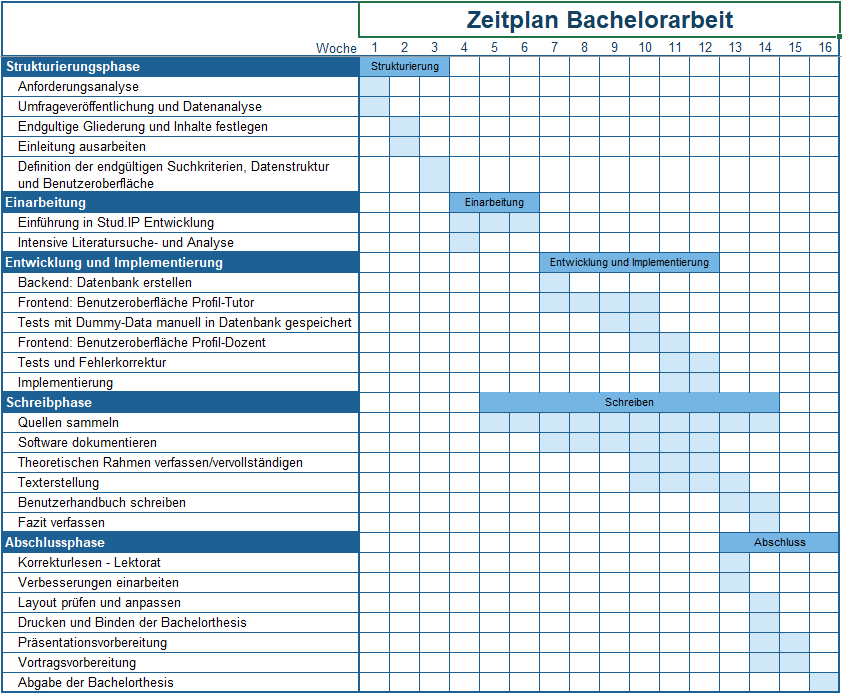
\includegraphics[height=12.5cm,keepaspectratio]{pics/zeitplan}\\
    \caption{Zeitplanung}
\end{figure}

\section{Abzuliefernde Ergebnisse}
\begin{itemize}
	\item schriftliche Ausarbeitung der Bachelorarbeit
	\item CD-ROM mit:
	\begin{itemize}
		\item Programme
		\item Source-Code
		\item Benutzerhandbuch
		\item multimediale Supplementen
		\item Präsentationsfolien
	\end{itemize}
\end{itemize}



% Appendix
\begin{appendix}
\section{Anhang}
\captionsetup{list=no}
\setcounter{figure}{0}

\begin{figure}[hp]%[H]
    \centering
    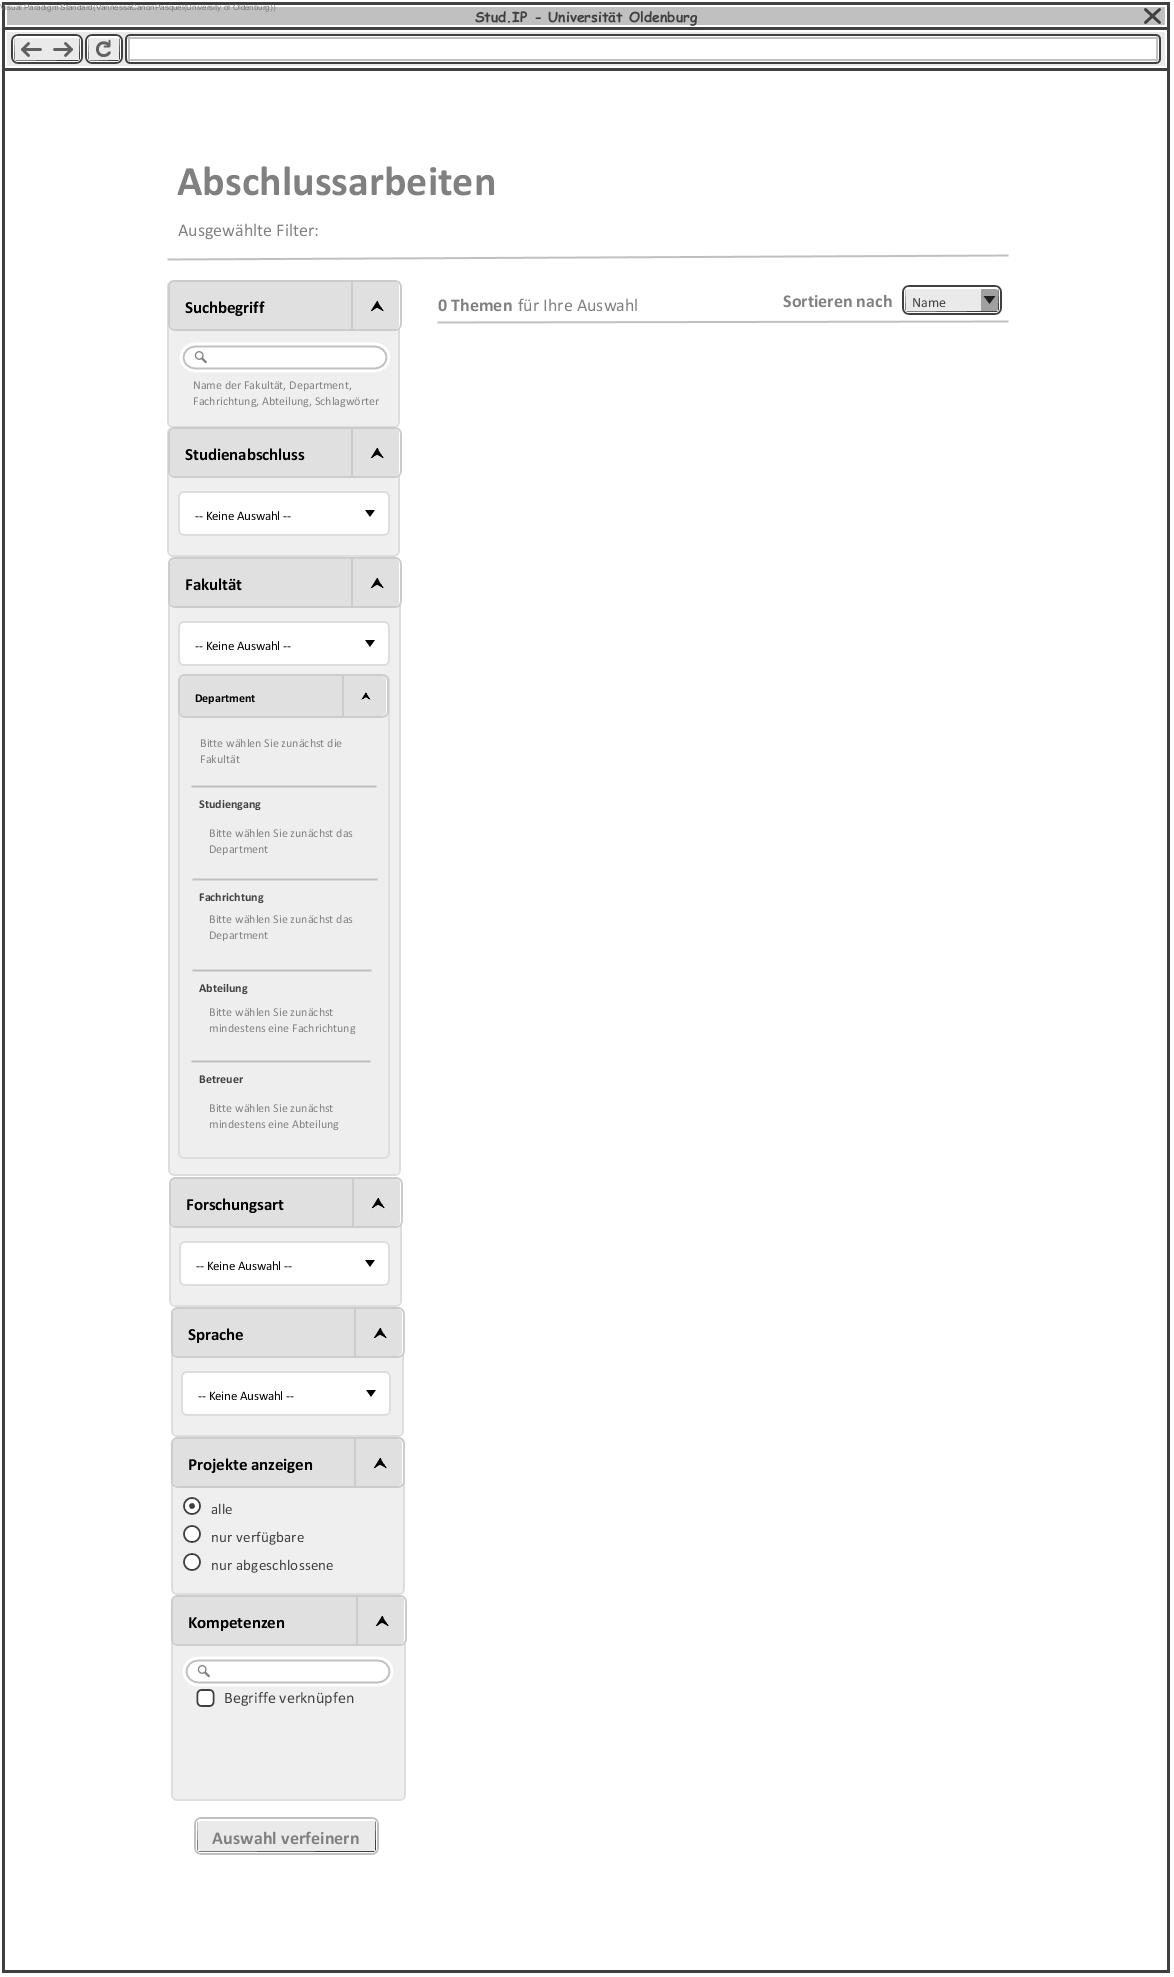
\includegraphics[height=15cm,keepaspectratio]{pics/anhang_a/Expanded}\\
    \caption{Erste Maske}
\end{figure}
\cleardoublepage

\begin{figure}[hp]%[H]
    \centering
    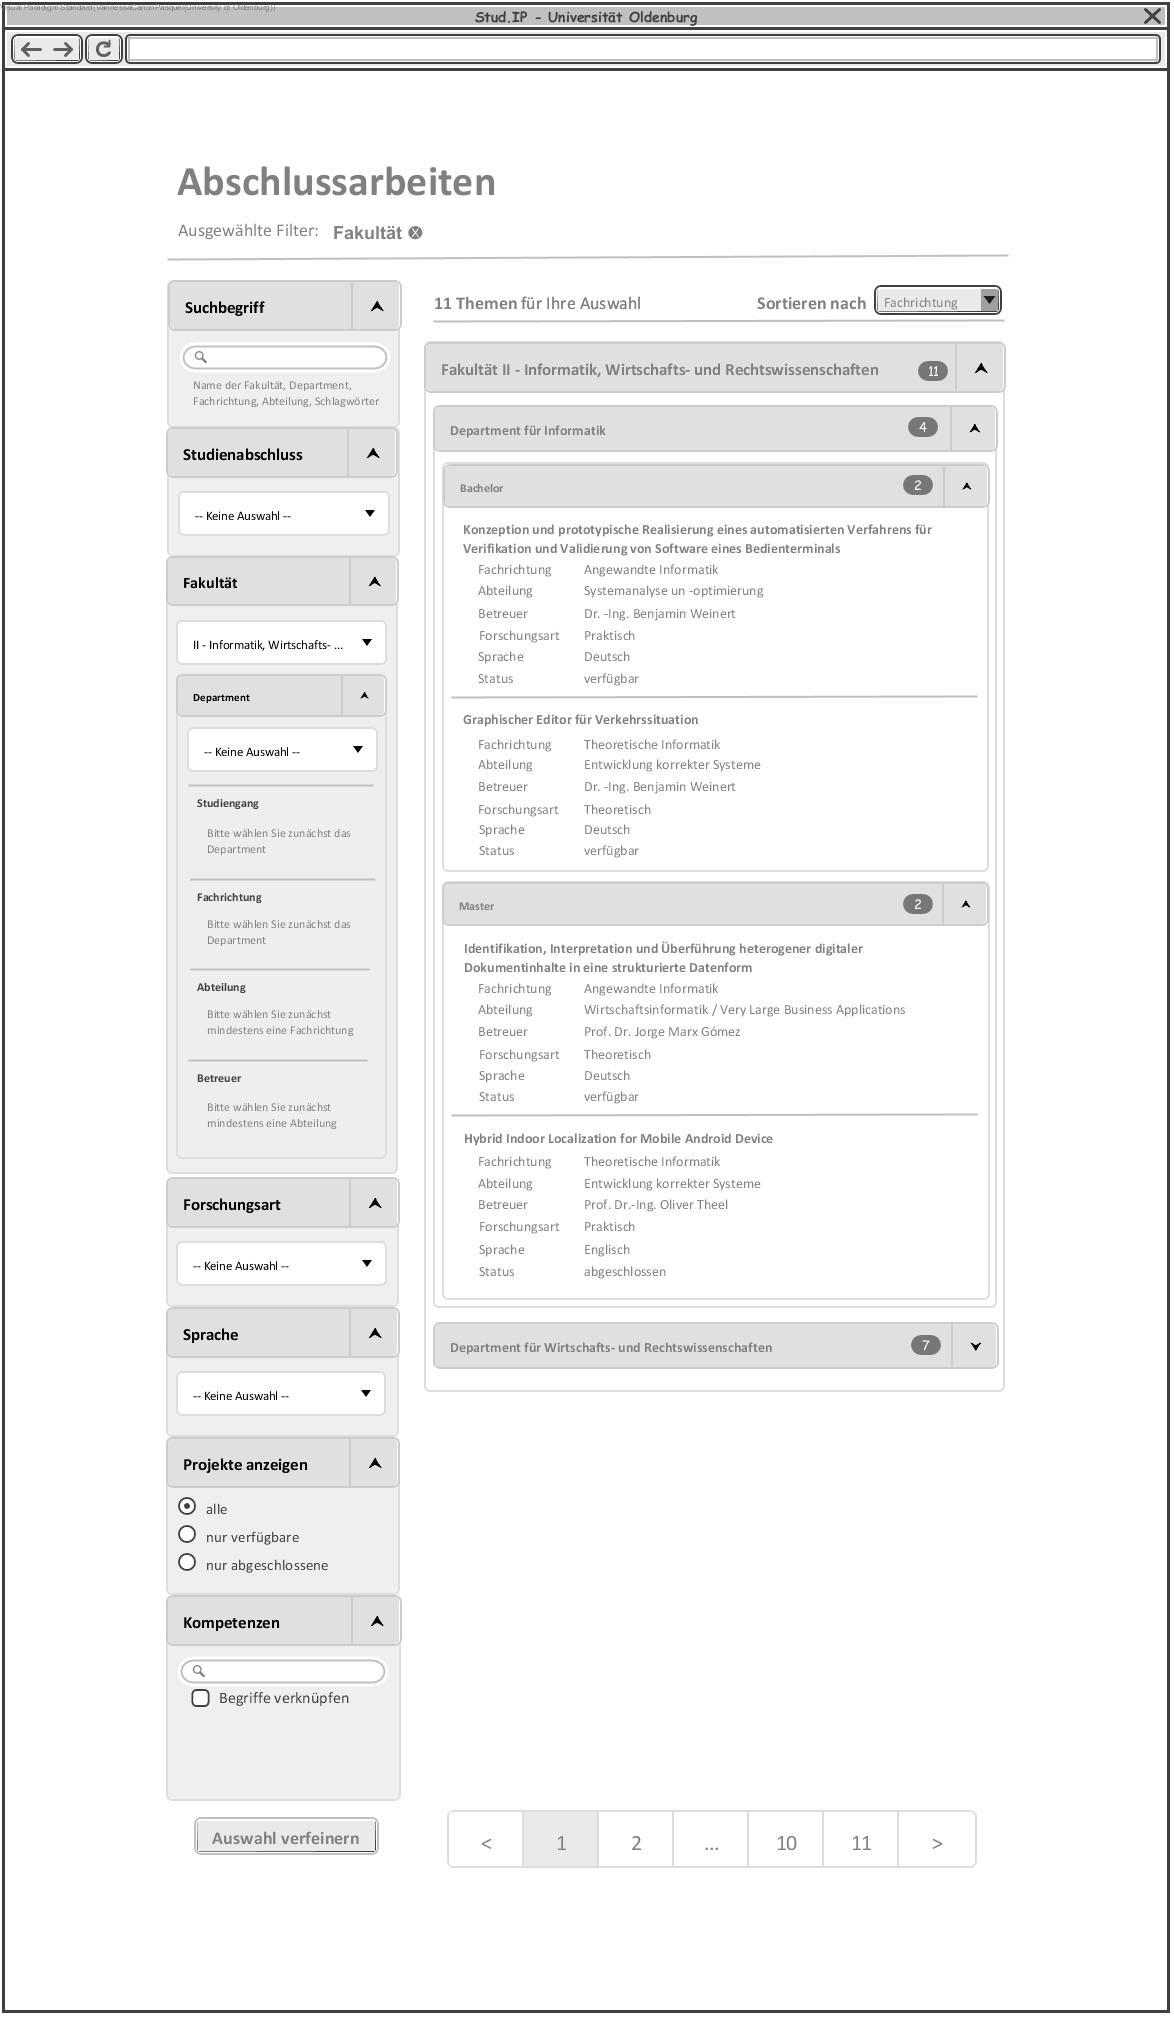
\includegraphics[height=20cm,keepaspectratio]{pics/anhang_a/FakII}\\
    \caption{Verfeinern nach Fakultät}
\end{figure}
\cleardoublepage

\begin{figure}[hp]%[H]
    \centering
    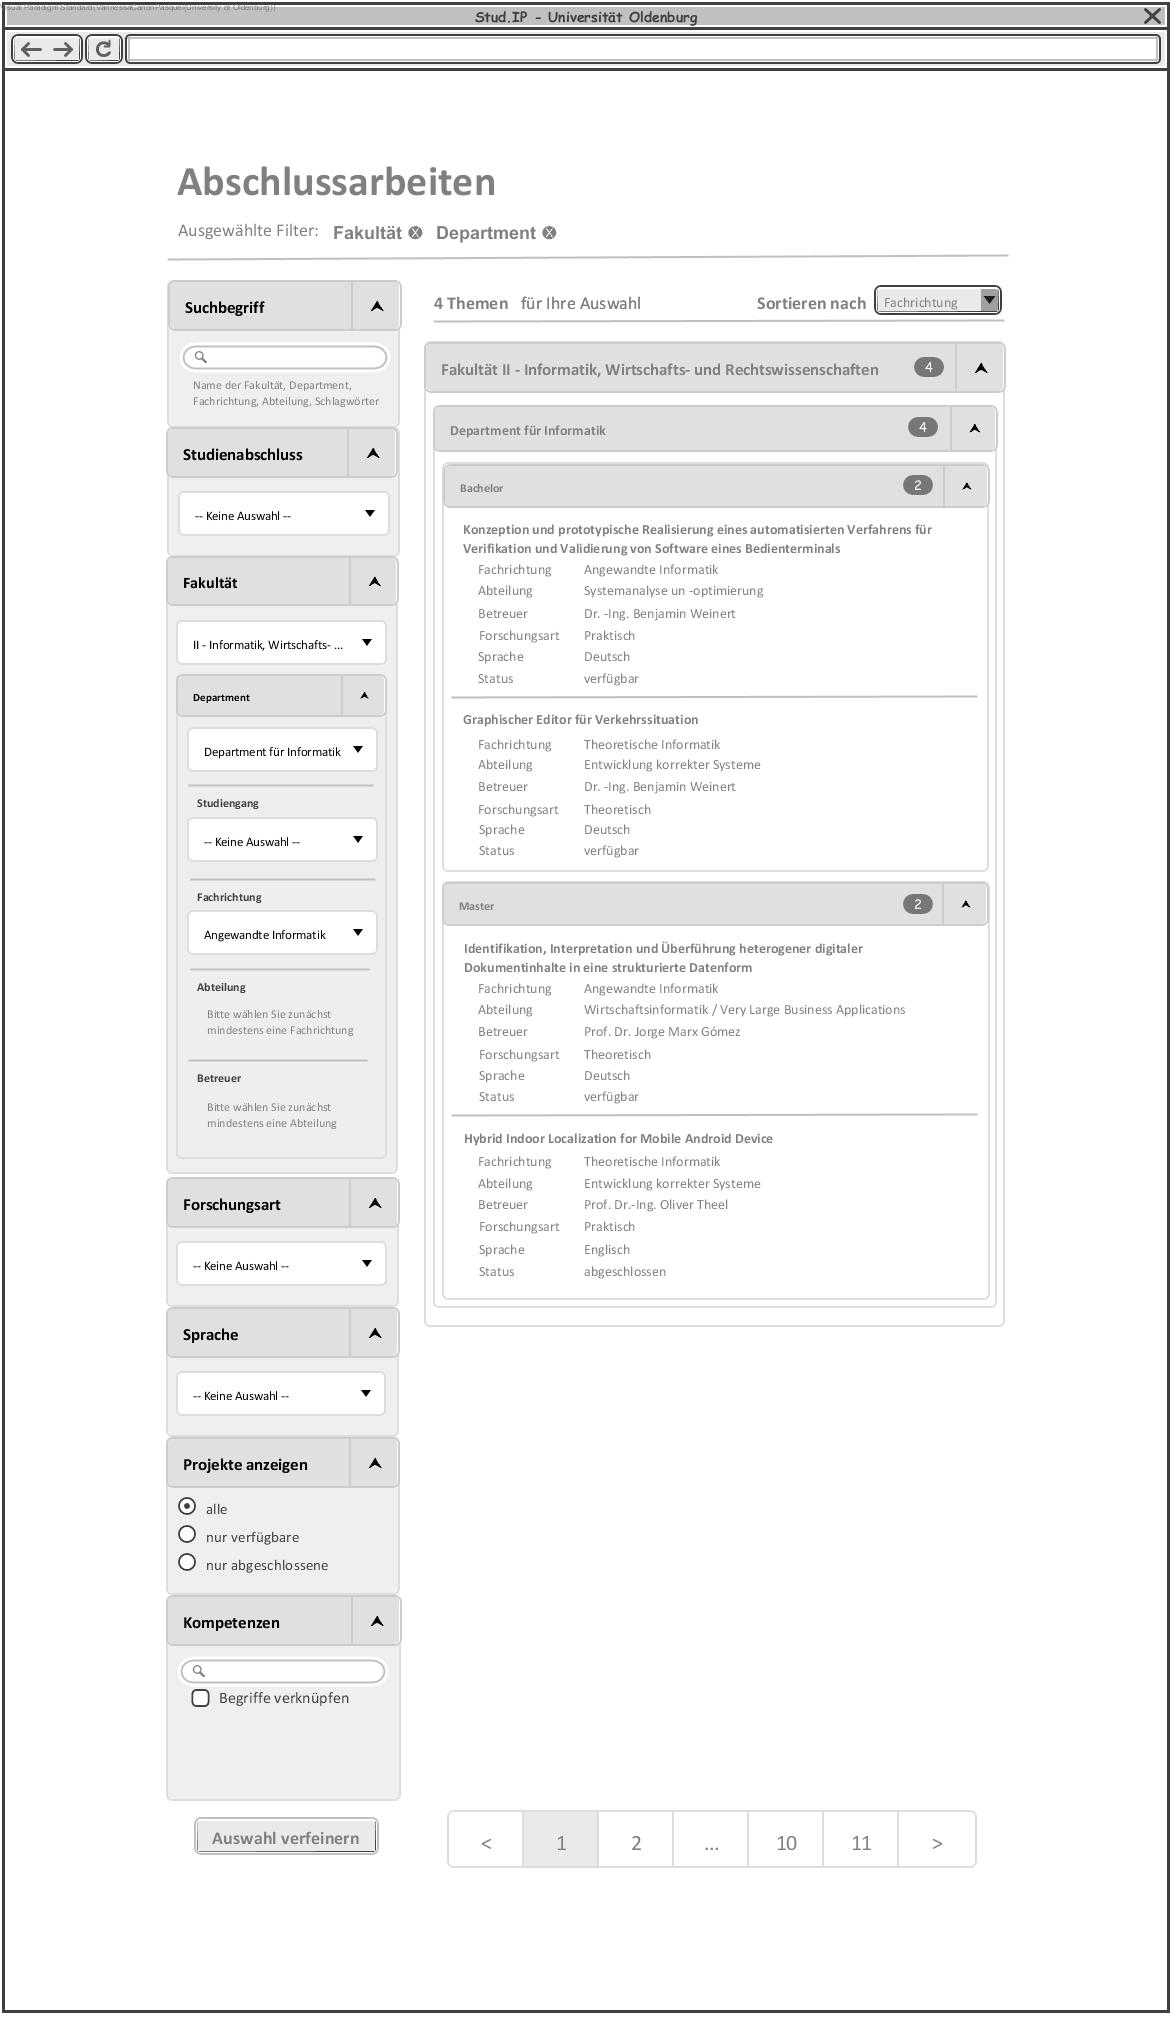
\includegraphics[height=20cm,keepaspectratio]{pics/anhang_a/DfI}\\
    \caption{Verfeinern nach Fakultät - Department}
\end{figure}
\cleardoublepage

\begin{figure}[hp]%[H]
    \centering
    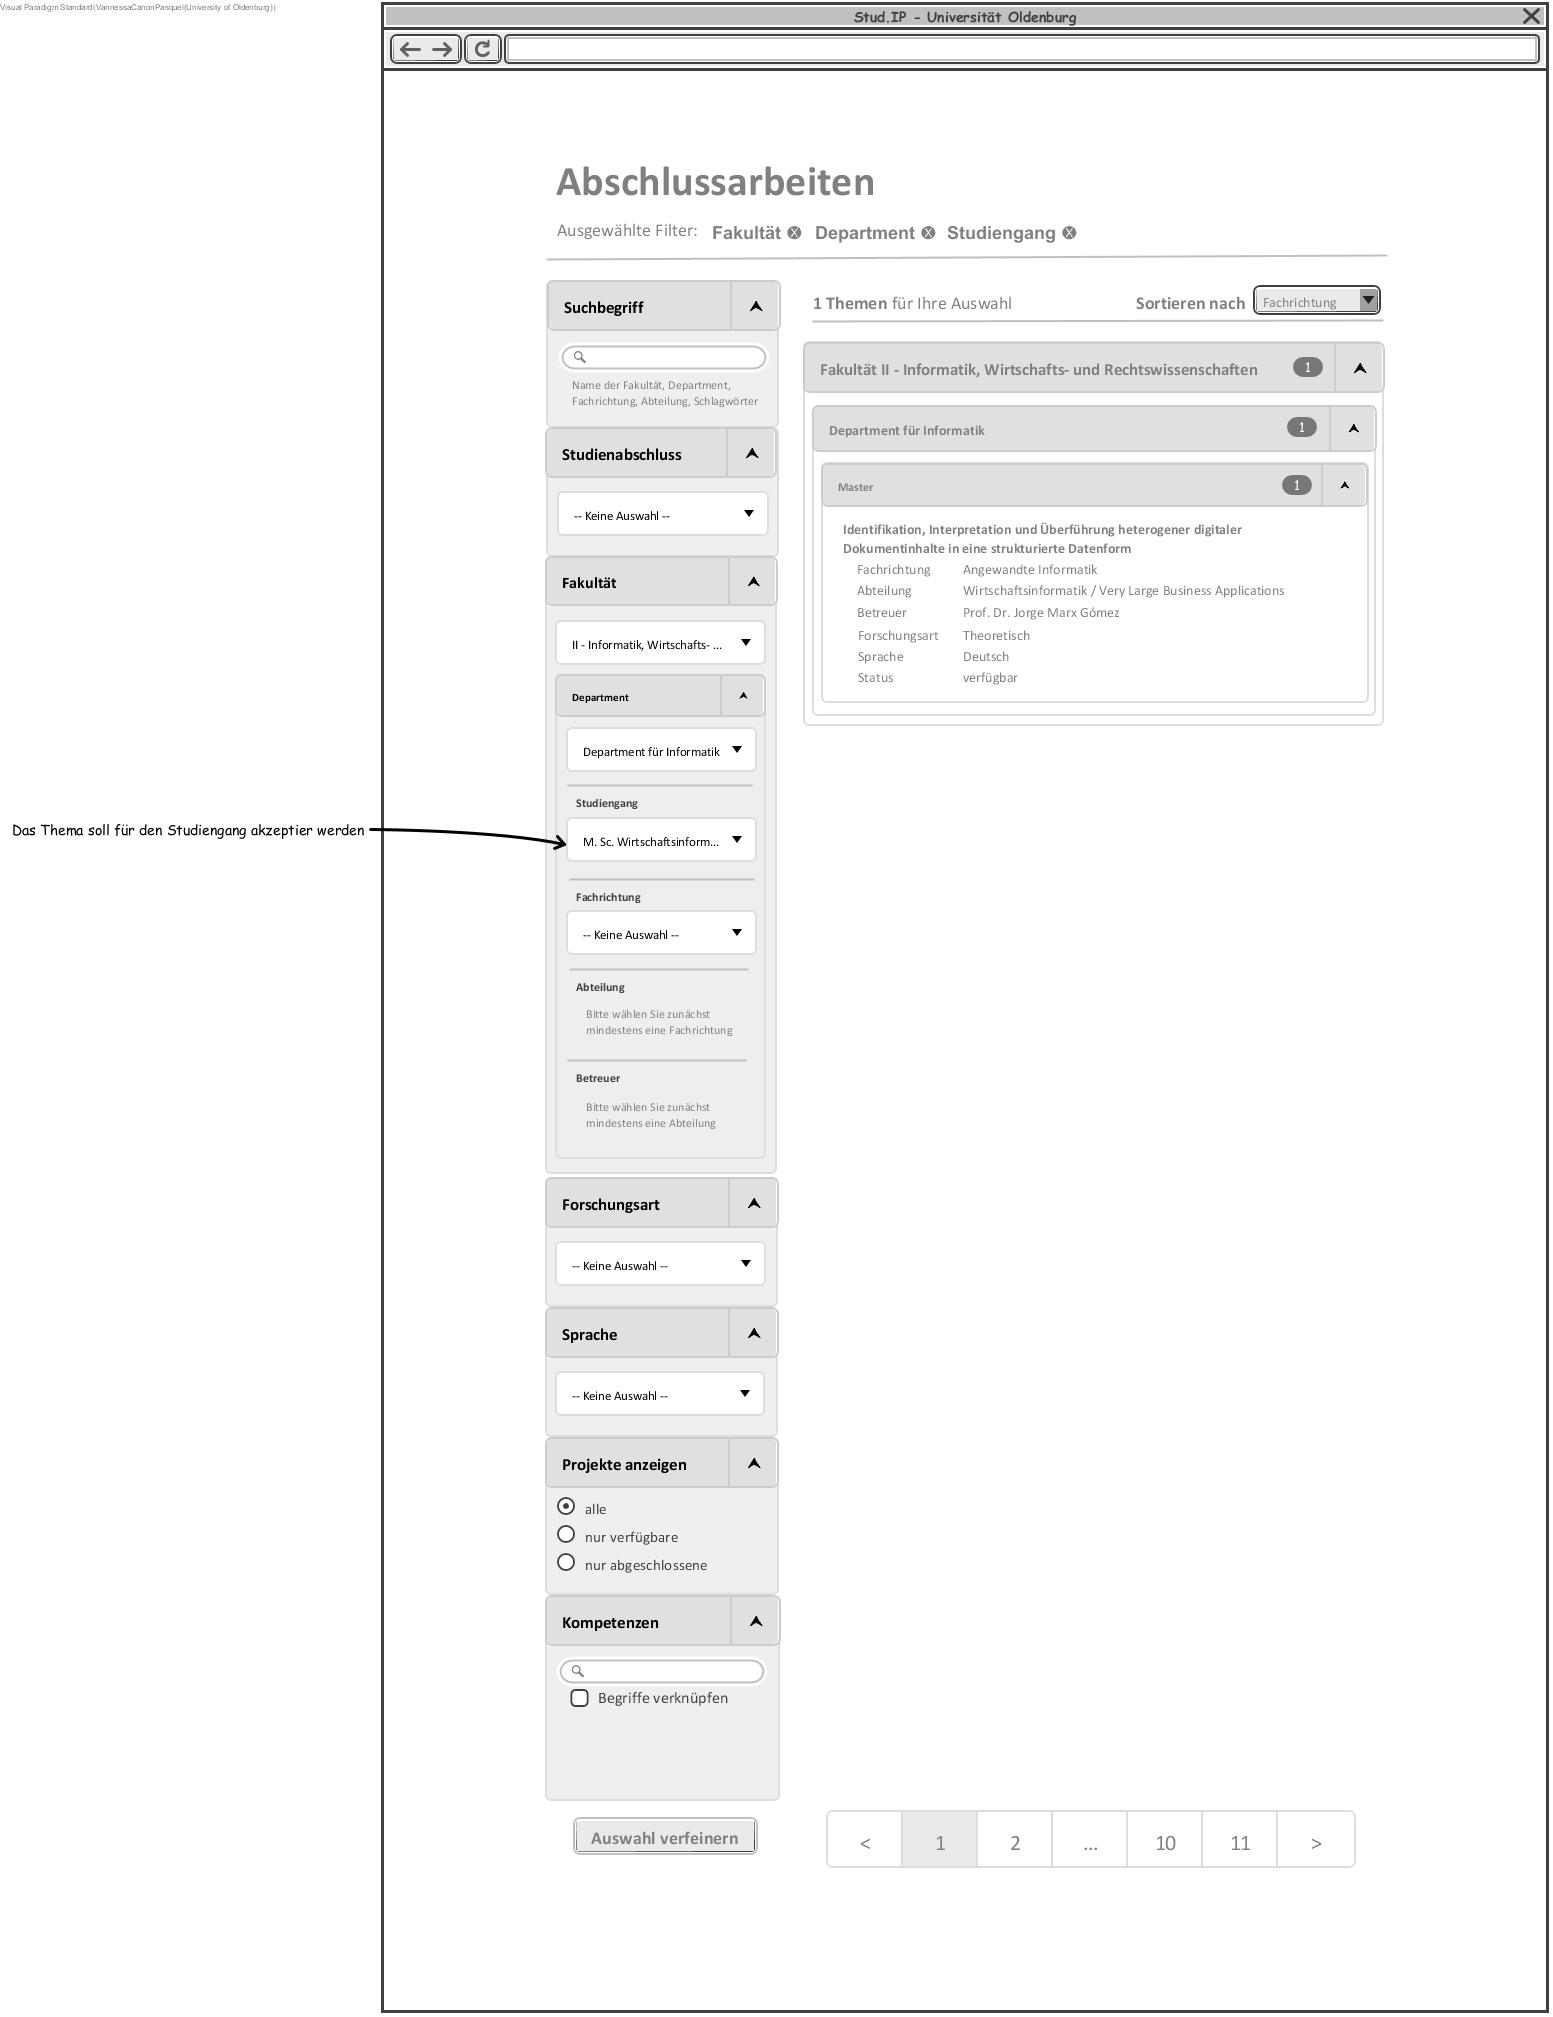
\includegraphics[height=20cm,keepaspectratio]{pics/anhang_a/Studiengang}\\
    \caption{Verfeinern nach Fakultät – Department - Studiengang}
\end{figure}
\cleardoublepage

\begin{figure}[hp]%[H]
    \centering
    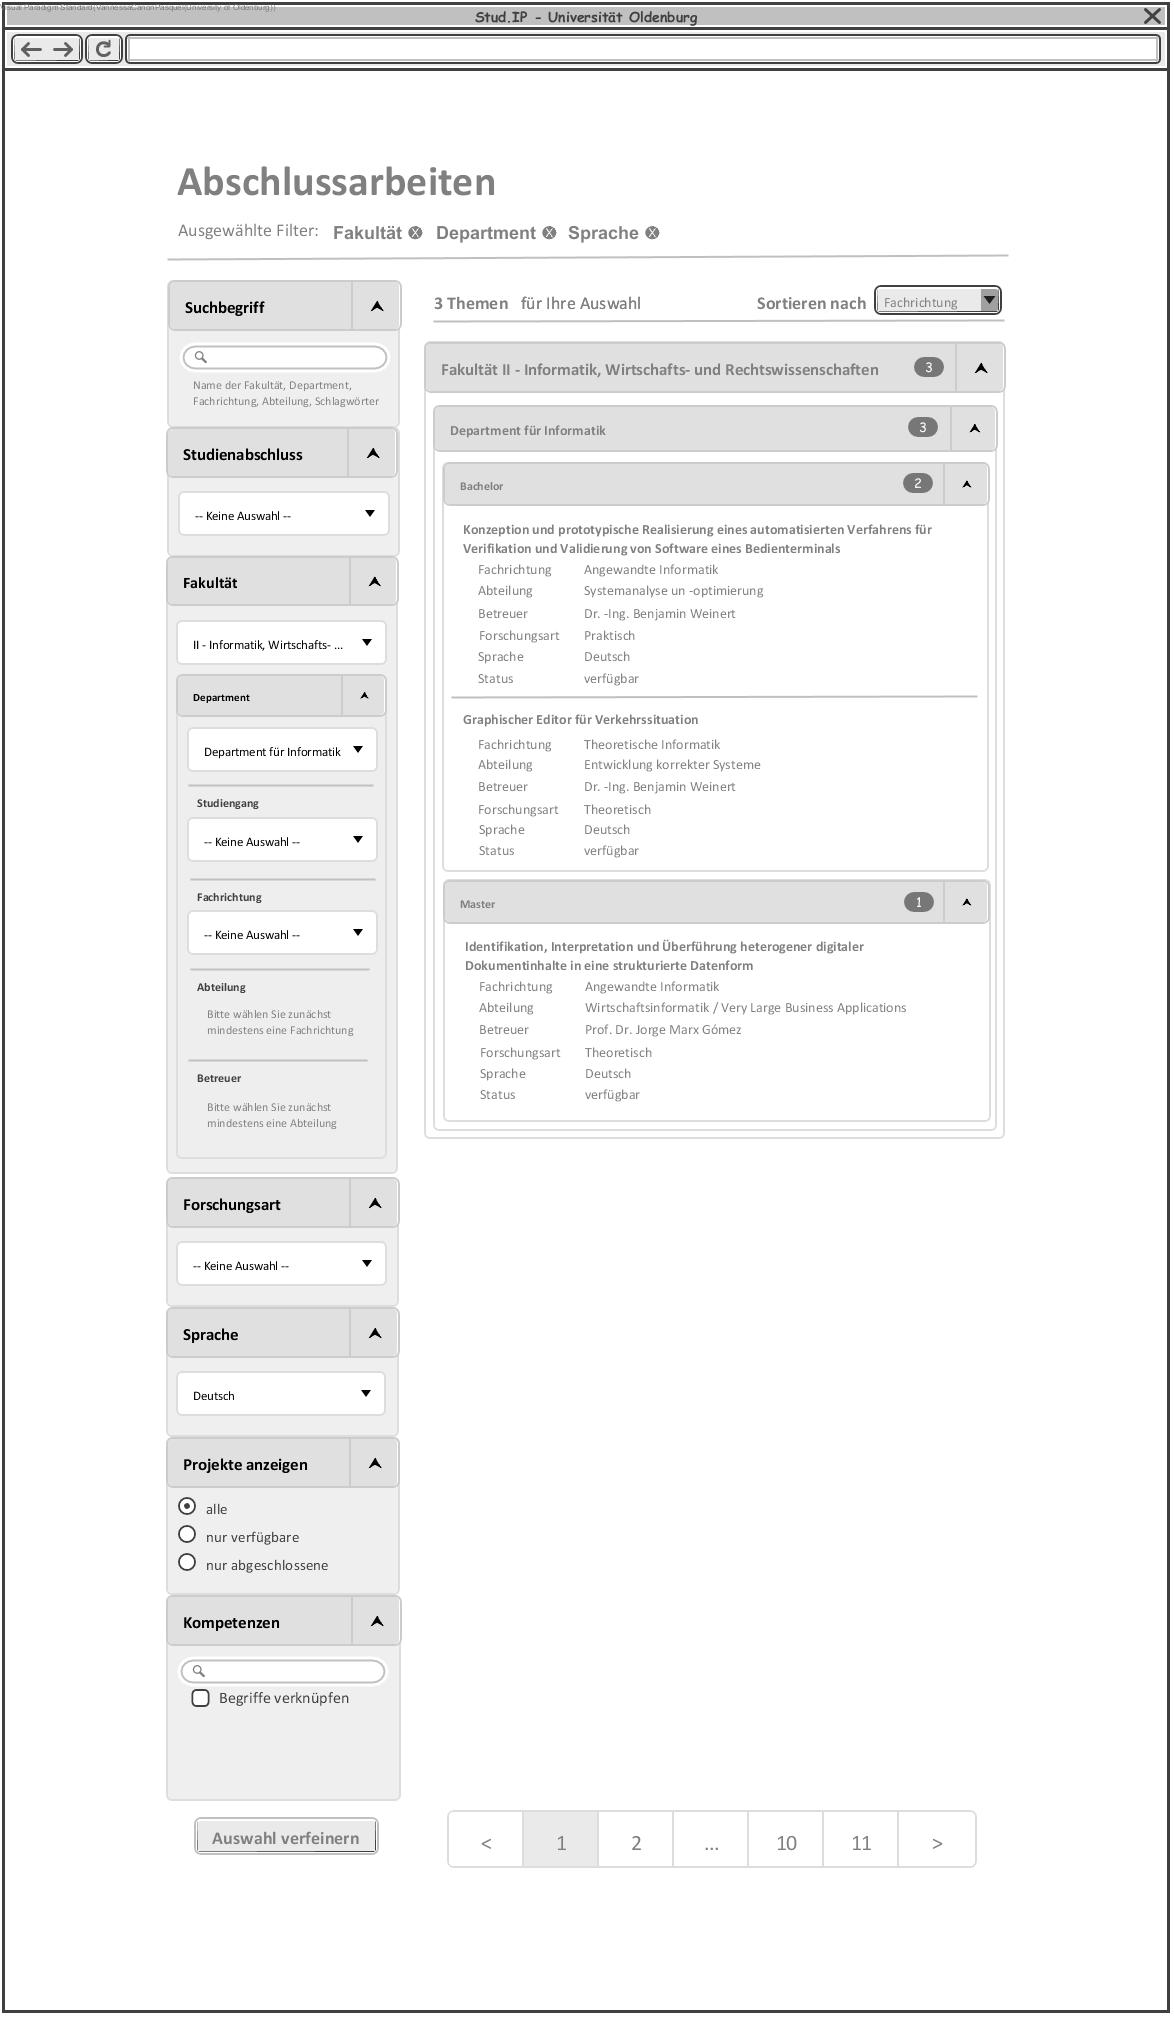
\includegraphics[height=20cm,keepaspectratio]{pics/anhang_a/Sprache}\\
    \caption{Verfeinern nach Fakultät – Department - Sprache}
\end{figure}
\cleardoublepage

\begin{figure}[hp]%[H]
    \centering
    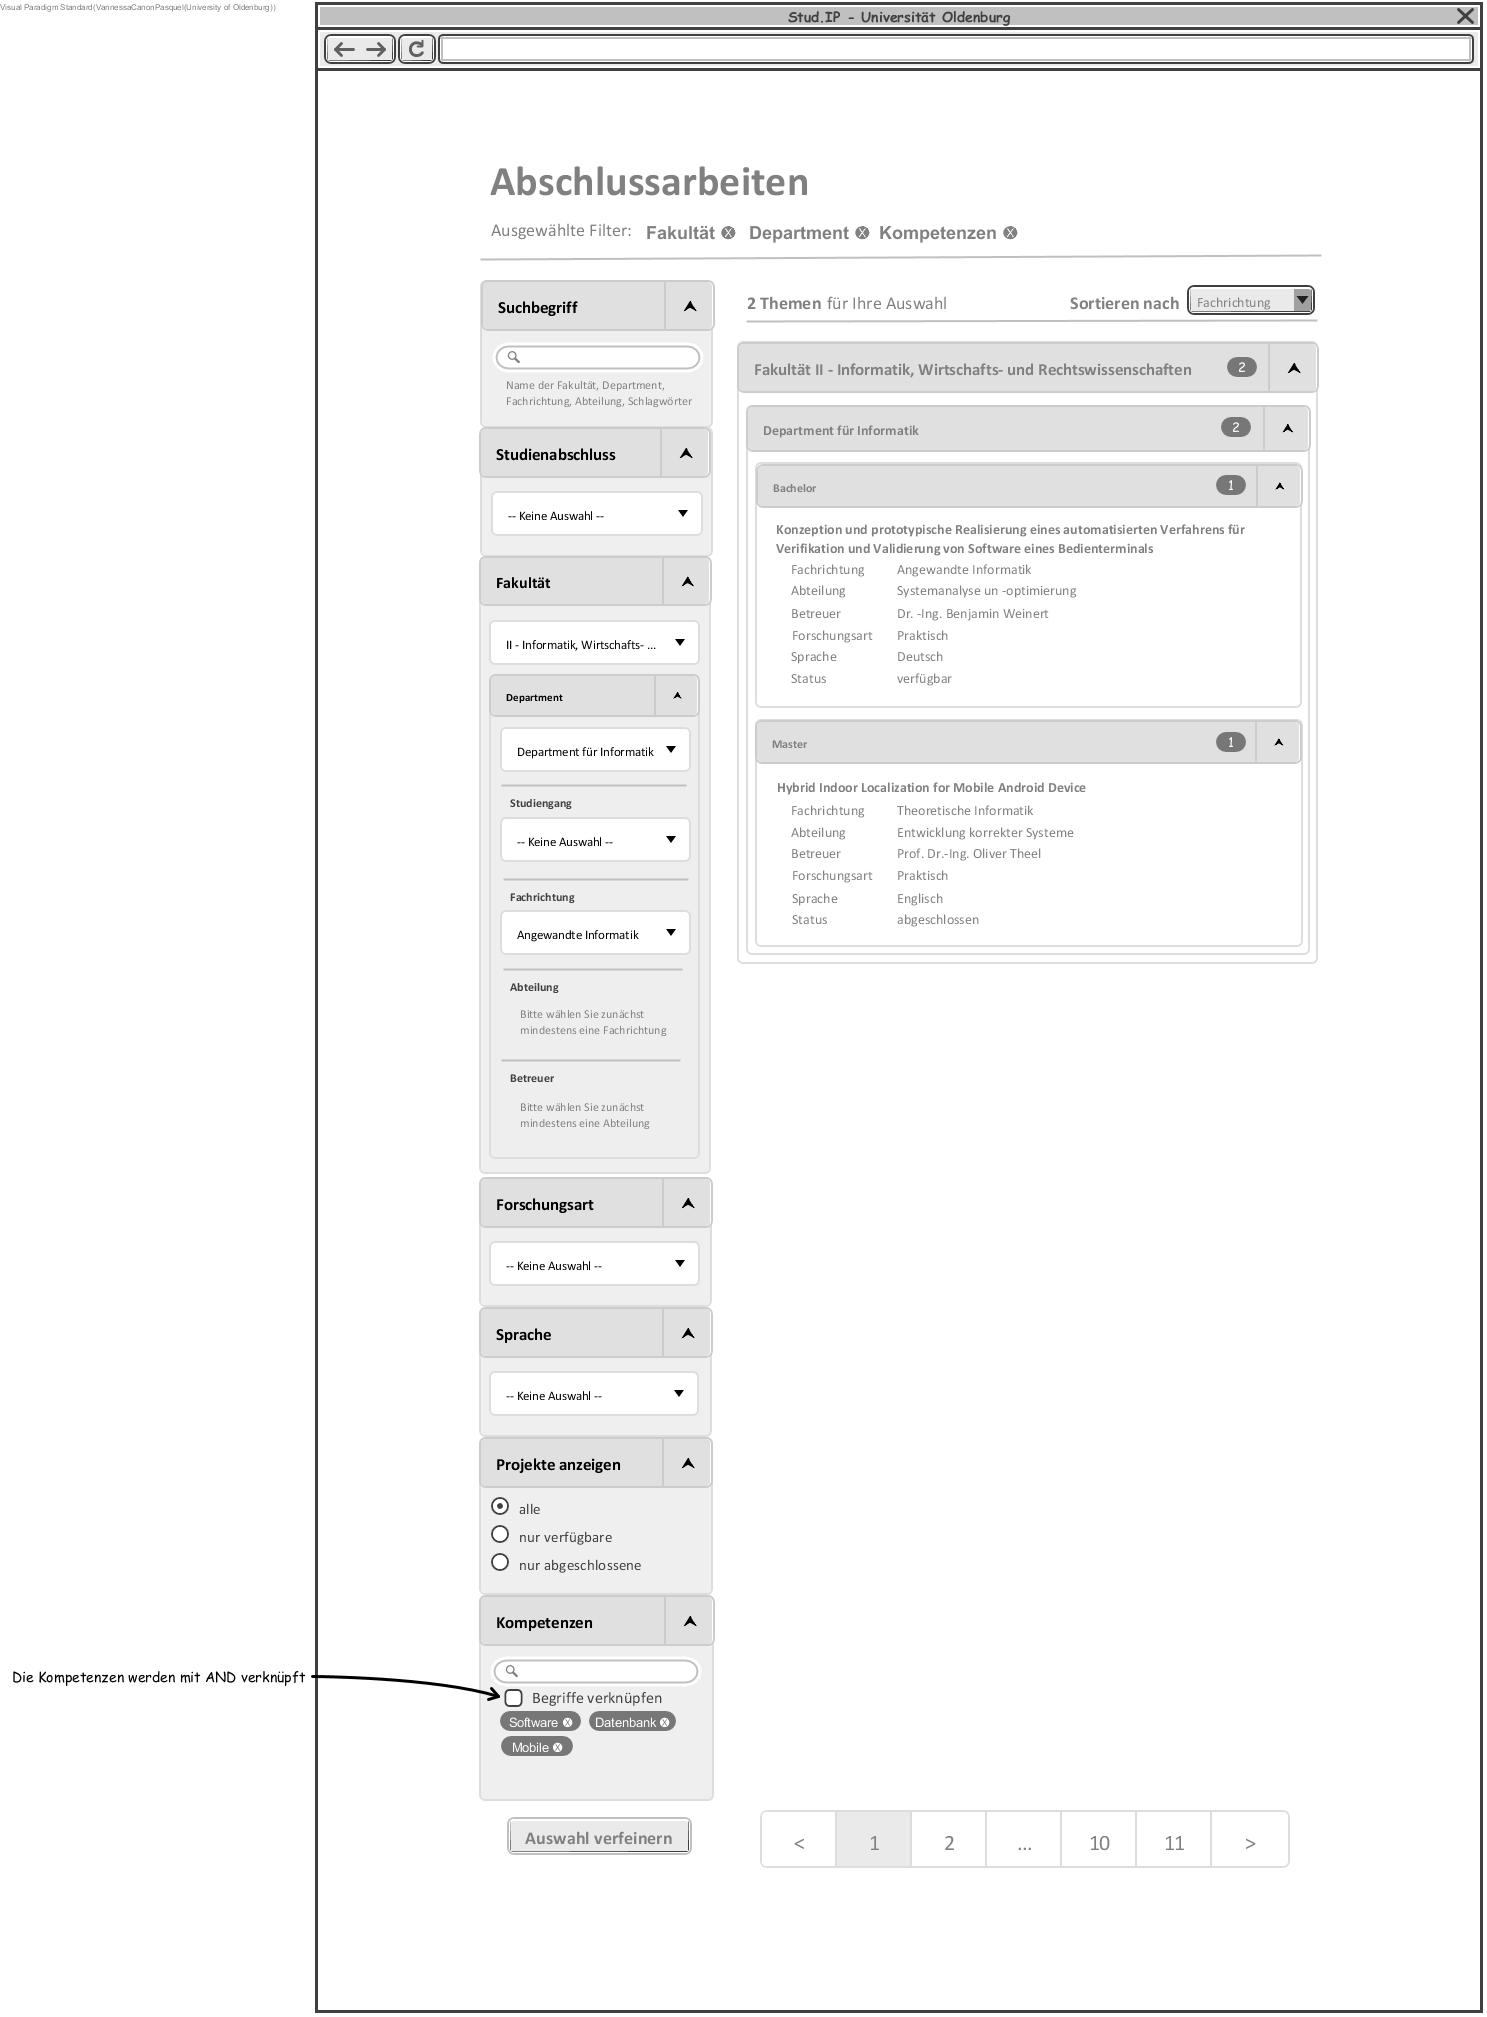
\includegraphics[height=20cm,keepaspectratio]{pics/anhang_a/Kompetenzen}\\
    \caption{Verfeinern nach Fakultät – Department - Kompetenzen}
\end{figure}
\cleardoublepage

\begin{figure}[hp]%[H]
    \centering
    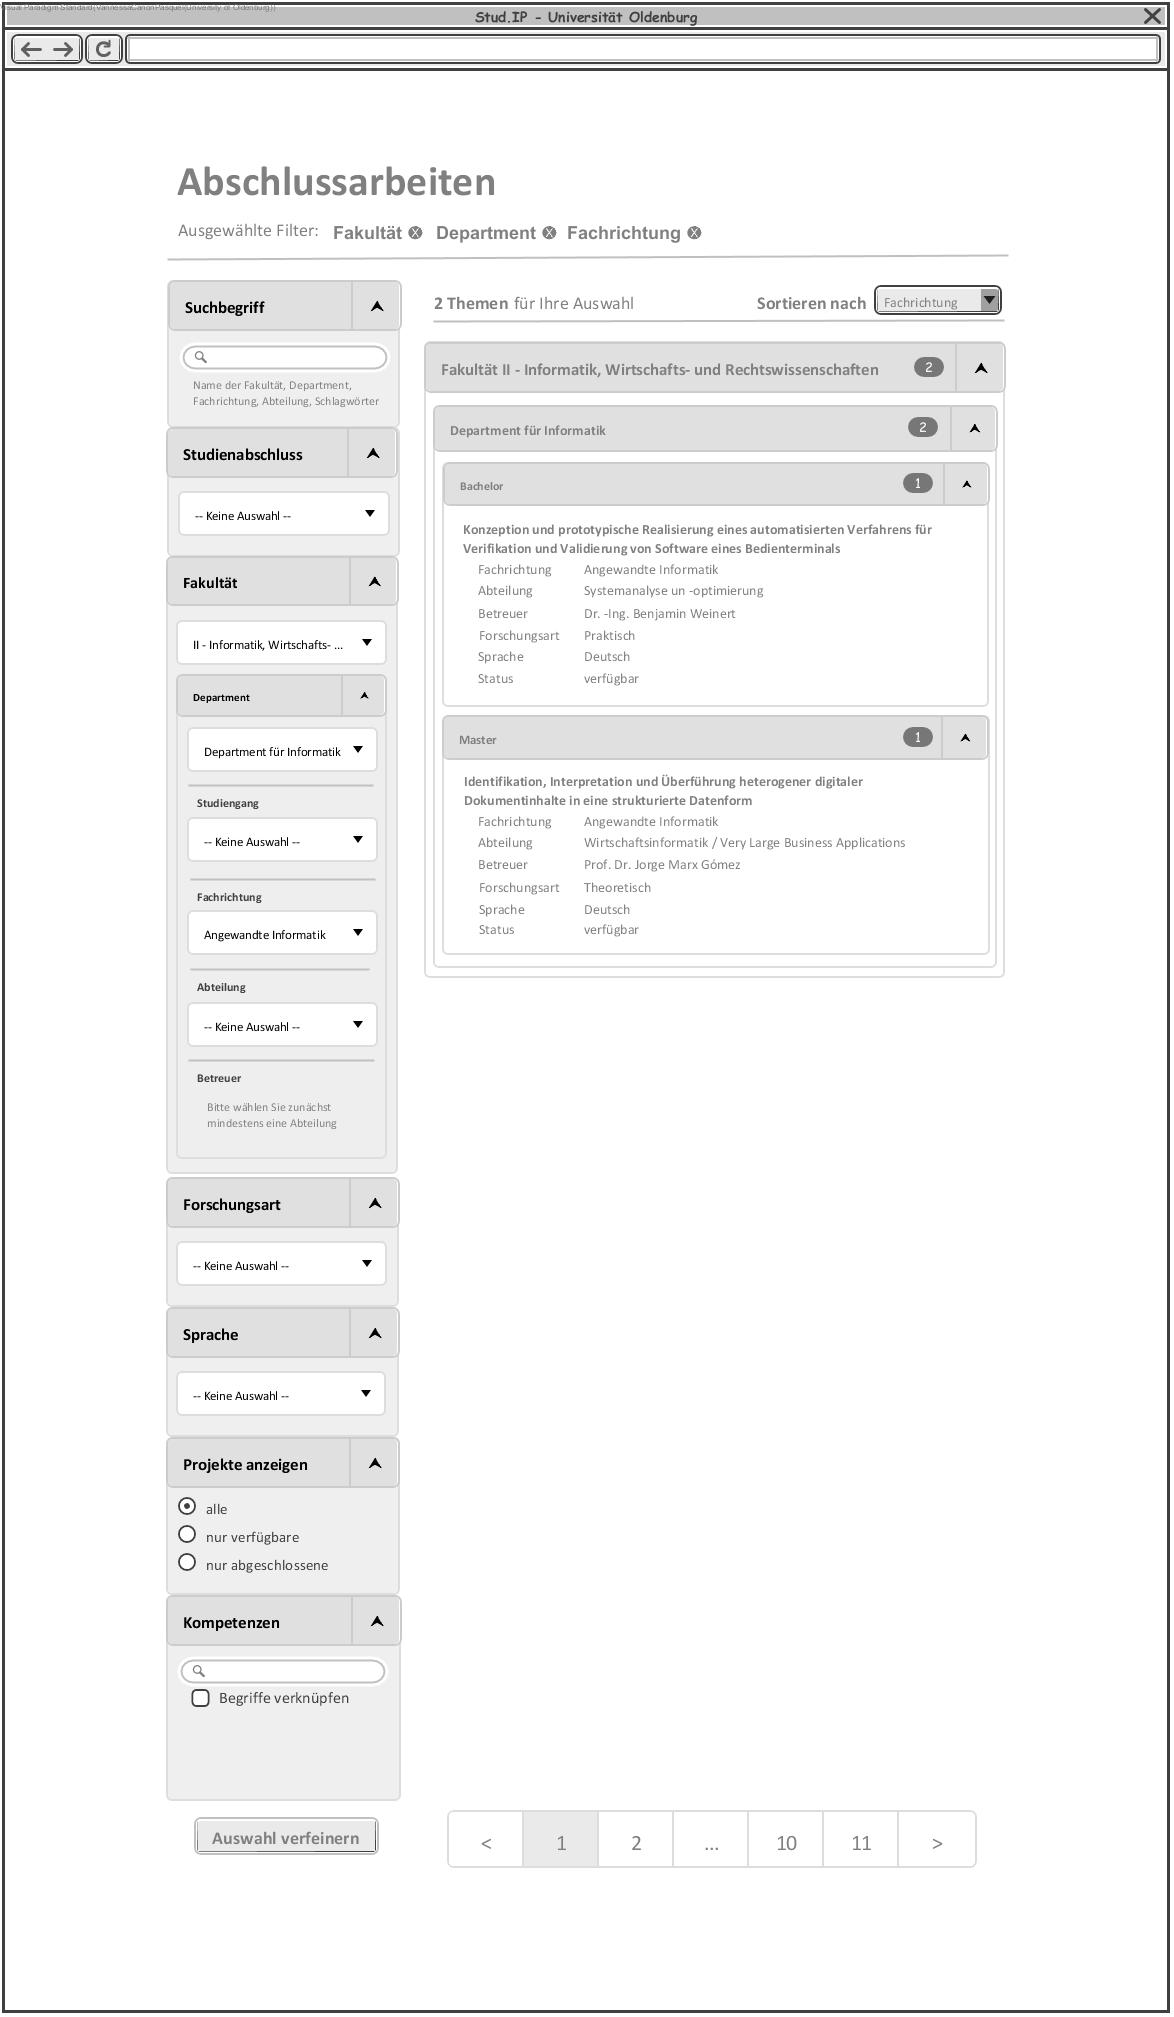
\includegraphics[height=20cm,keepaspectratio]{pics/anhang_a/Fachrichtung}\\
    \caption{Verfeinern nach Fakultät – Department - Fachrichtung}
\end{figure}
\cleardoublepage

\begin{figure}[hp]%[H]
    \centering
    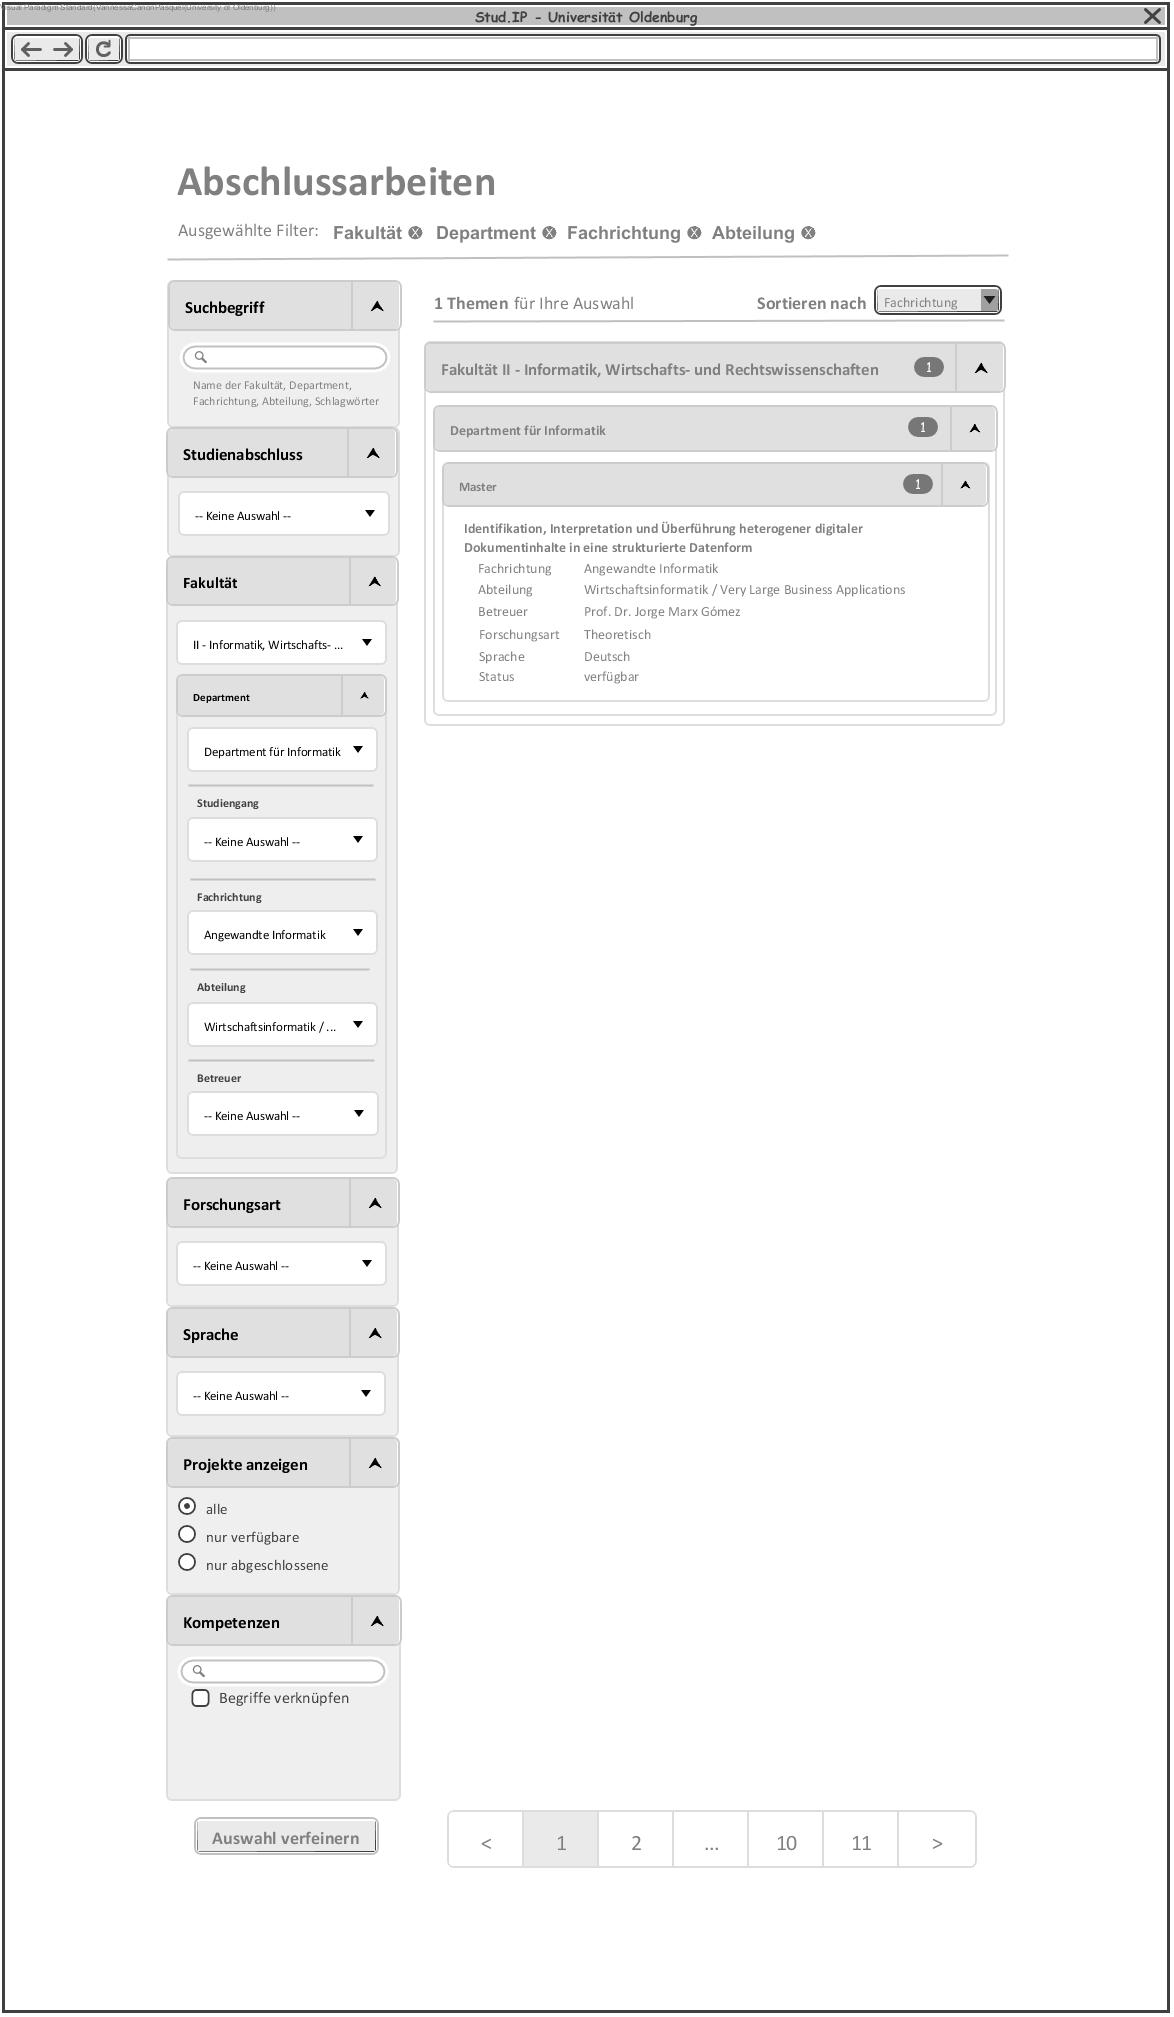
\includegraphics[height=20cm,keepaspectratio]{pics/anhang_a/Abteilung}\\
    \caption{Verfeinern nach Fakultät – Department – Fachrichtung - Abteilung}
\end{figure}
\cleardoublepage

\begin{figure}[hp]%[H]
    \centering
    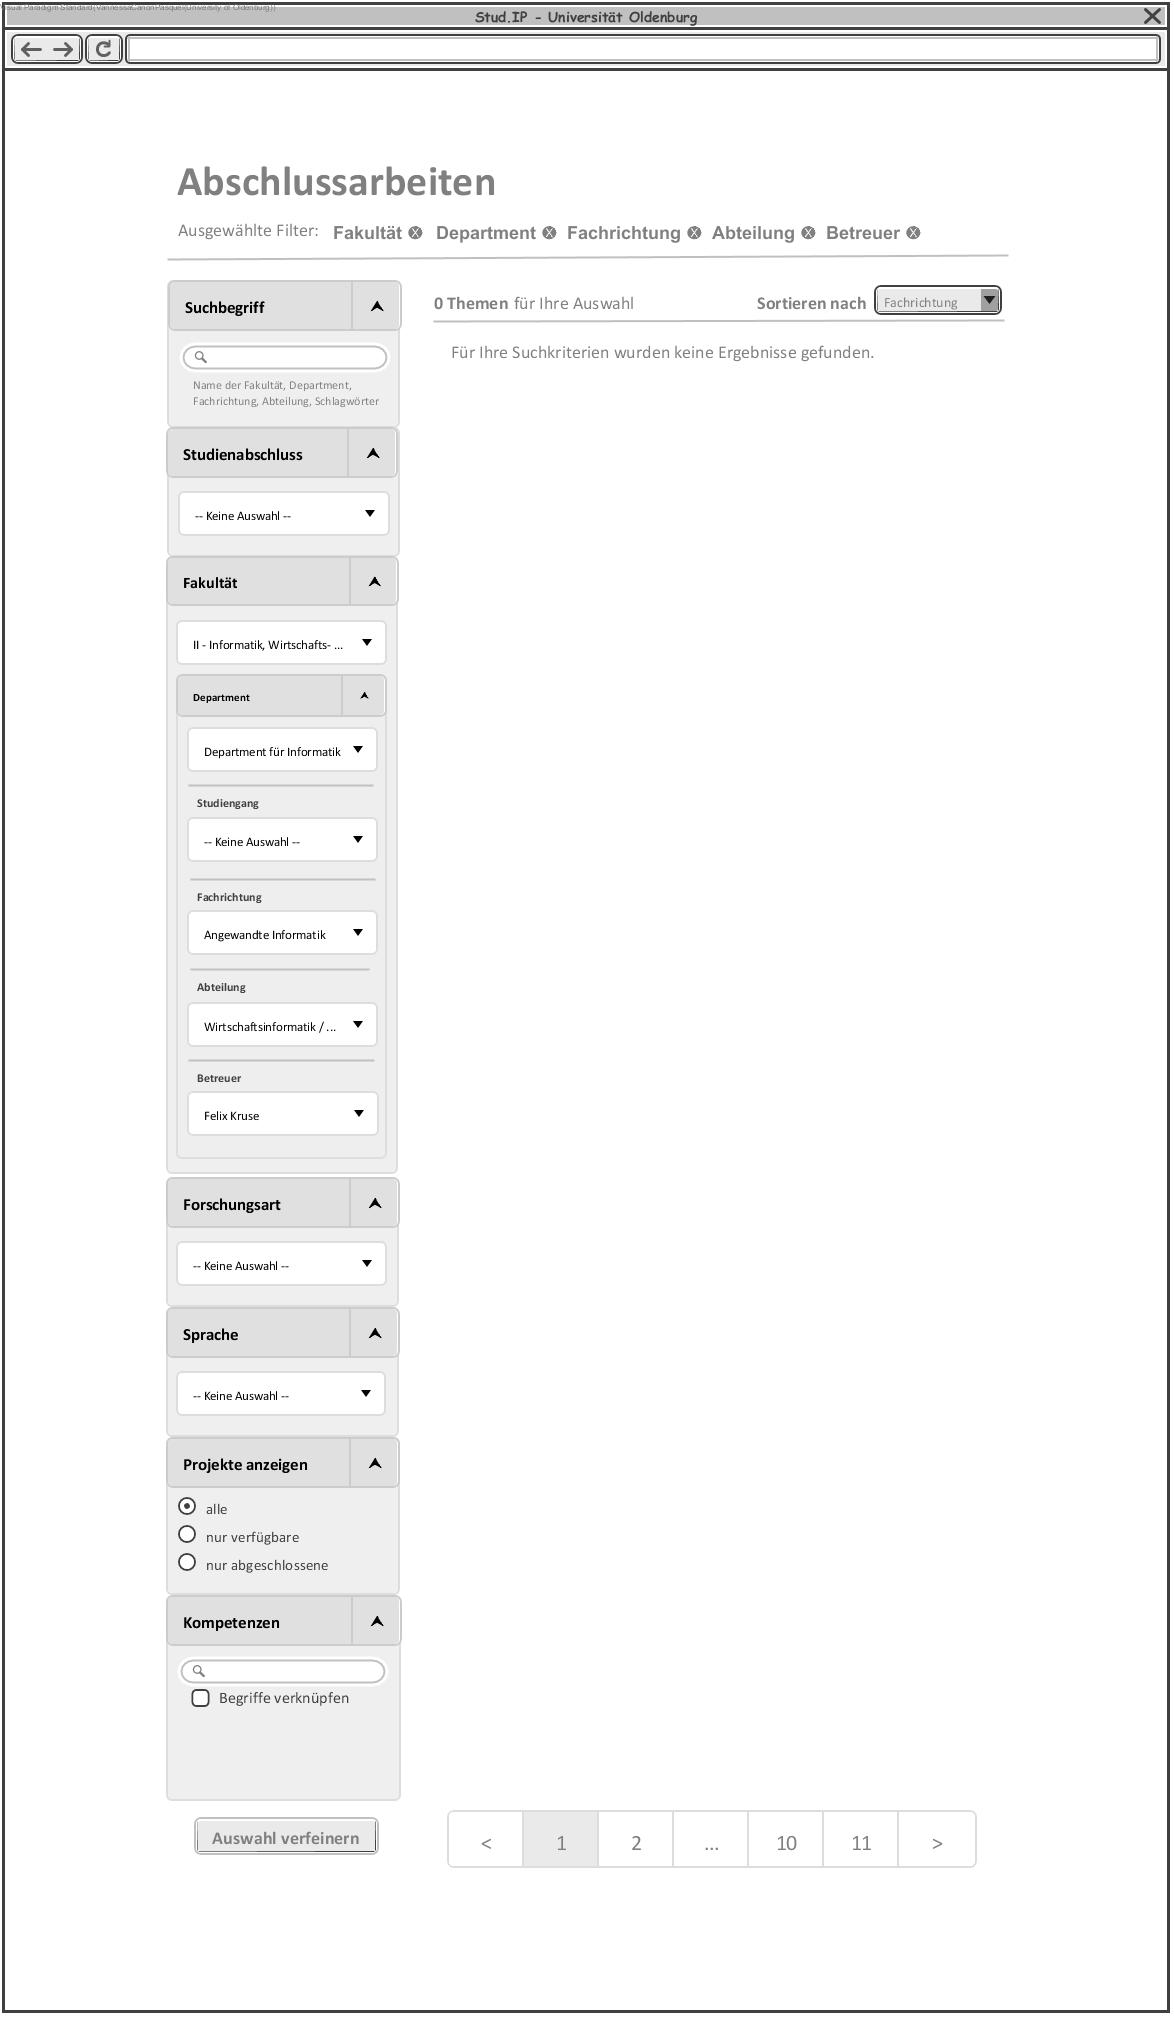
\includegraphics[height=20cm,keepaspectratio]{pics/anhang_a/Betreuer}\\
    \caption{Verfeinern nach Fakultät – Department – Fachrichtung - \\Abteilung - Betreuer}
\end{figure}


%\begin{verbatim}
%10 PRINT "Sales and Distribution"
%20 GOTO 10
%\end{verbatim}

\newpage
\addcontentsline{toc}{section}{Literaturverzeichnis}
\bibliographystyle{alpha}
\bibliography{papers} % Point to BibTeX literature file e.g. literatur.bib

\end{appendix}

\end{document}
